\documentclass[a4paper, 14pt, oneside]{Thesis}
%\usepackage{ulem}
\usepackage[square, numbers, comma, sort&compress]{natbib}  % Use the "Natbib" style for the references in the Bibliography

\usepackage{pslatex} %To set the font as Times New Roman
\usepackage{amsbsy} 
\usepackage{amsfonts}
\usepackage{graphicx}
\usepackage{dcolumn}
\usepackage{amsmath}
\usepackage{latexsym}
\usepackage{amssymb}
\usepackage{epsfig}
\usepackage{verbatim} 
\usepackage{soul}
\bibliographystyle{apa}

\usepackage{epsfig,graphics}
\usepackage{amsmath, amsthm, amssymb}
\usepackage{subfigure}
\usepackage{tikz}
\usepackage{float}

\usepackage{graphicx}
\usepackage[export]{adjustbox}
%\usepackage{fancyhdr}
%\usepackage{lipsum}

%To have 1. instead of [1] in the bibliographic entry
\makeatletter
\renewcommand\@biblabel[1]{#1.}
\makeatother

% To remove hyphenation
\tolerance=1
\emergencystretch=\maxdimen
\hyphenpenalty=10000
\hbadness=10000
%
%----To make sure the page numbers are in the top middle of each page.
\fancypagestyle{Thesis}{
\fancyhf{}
\fancyhead[C]{\thepage}
\%lfoot{\thepage}
\pagestyle{fancy}
}
%redefine the plain pagestyle
%\fancypagestyle{plain}{
%\fancyhf{}
%\fancyhead[C]{\thepage}
%}
%----------------------------------------------------------------------
%% ------------------------s----------------------------------------
% Some new environments for the paper
%
\newtheorem{dfn}{Definition}[section]
\newtheorem{prop}[dfn]{Proposition}
\newtheorem{lem}[dfn]{Lemma}
\newtheorem{thm}[dfn]{Theorem}
\newtheorem{cor}[dfn]{Corollary}
\newtheorem{clm}[dfn]{Claim}
\newtheorem{fact}[dfn]{Fact}
%
%\newcommand{\RightBox}{\begin{flushright} $\Box$ \end{flushright}}
\newcommand{\RightBox}{{\phantom{a}}\hfill $\Box$ \\}
%\newenvironment{proof}{{\bf Proof:~}}{\RightBox}
\newenvironment{prf}{{\bf Proof~Idea:~}}{\RightBox}
%\newcommand{\claim}[1]{{\bf Claim #1:~}}
%
\newcommand{\Dfn}[1]{Definition \ref{dfn:#1}}
\newcommand{\Prop}[1]{Proposition \ref{prop:#1}}
\newcommand{\Lem}[1]{Lemma \ref{lem:#1}}
\newcommand{\Thm}[1]{Theorem \ref{thm:#1}}
\newcommand{\Cor}[1]{Corollary \ref{cor:#1}}

%Action-indexed diamond modality
\newcommand{\Adiam}[1]{\mbox{$\langle #1 \rangle$}}
\newcommand{\diamin}{\Diamond\kern-0.5em{\raisebox{.25ex}{\rm -}}\kern0.175em}
\newcommand{\until}{\mbox{\large\bf U}}
\newcommand{\since}{\mbox{\large\bf S}}
\newcommand{\nxt}{\mbox{$\bigcirc$}}
\newcommand{\nxtdot}{\displaystyle \bigodot}
\newcommand{\past}{\diamin}
\newcommand{\ifpast}{\mbox{$\boxminus$}}
\newcommand{\now}{\mbox{$\langle now \rangle$}}
\newcommand{\Now}{\mbox{$[now]$}}
\newcommand{\pres}{\mbox{$\rangle \langle$}}
\newcommand{\snd}{\mbox{\large\bf s}}
\newcommand{\rec}{\mbox{\large\bf r}}
\newcommand{\nc}{\mathbf{no\_comm}}

%Propositional connectives
%\newcommand{\implies}{{\raisebox{.20ex}{$\scriptstyle ~\supset~$}}}
\newcommand{\Not}{\mbox{$\lnot$}}
\newcommand{\xor}{\oplus}
\newcommand{\True}{\mathit{True}}
\newcommand{\False}{\mathit{False}}
\newcommand{\Imply}{\supset}
%Large symbols
\newcommand{\andover}{\displaystyle \bigwedge}
\newcommand{\orover}{\displaystyle \bigvee}
\newcommand{\capover}{\displaystyle \bigcap}
\newcommand{\cupover}{\displaystyle \bigcup}
\newcommand{\piover}{\displaystyle \Pi}
\newcommand{\ohat}[1]{\widehat{#1}}
\newcommand{\otilde}[1]{\widetilde{#1}}
\newcommand{\obar}[1]{\overline{#1}}
\newcommand{\Sigtil}{\mbox{$\otilde{\Sigma}$}}
\newcommand{\DA}{\mbox{$\Sigtil~=~(\Sigma_1, \dots, \Sigma_n)$}}

%Useful symbols
\newcommand{\derives}{\vdash}
\newcommand{\defn}{\mbox{$~\stackrel{\rm def}{=}~$}}
\newcommand{\qneq}{\mbox{$~\stackrel{\rm ?}{=}~$}}
\newcommand{\eqv}{\approx}
\newcommand{\hash}{\sharp}
\newcommand{\restr}{\lceil}
%\newcommand{\bot}{\bottom}
\newcommand{\nat}{{\bf N}}
\newcommand{\pfin}[1]{\mbox{$\wp_{fin}(#1)$}}
%\newcommand{\mod}[1]{\mbox{$|#1|$}}
\newcommand{\memb}[2]{\mbox{${#1} \in {#2}$}}
\newcommand{\E}{\mathbf{E}}



%Some roman words in math mode
\newcommand{\Iff}{\mbox{~iff~}}
\newcommand{\For}{\mbox{~for~}}
\newcommand{\Where}{\mbox{~where~}}
%\newcommand{\And}{\mbox{~and~}}
\newcommand{\Implies}{\mbox{~implies~}}

%Relations

% structures
\newcommand{\Sigstr}{\mbox{$\Sigma^*$}}
\newcommand{\TS}{\mbox{$TS = (Q,\to)$}}  %generates TS=(Q,->)
\newcommand{\TSP}{\mbox{$TS = (Q,\To)$}}         %generates TS=(Q,=>)
\newcommand{\TSi}{\mbox{$TS_i = (Q_i,\to_i)$}}           
\newcommand{\TSE}{\mbox{$TS_{ES}$}}
\newcommand{\TSN}{\mbox{$TS_{\cal N}$}}
\newcommand{\ES}{\mbox{$ES = (E,\leq,\#)$}}       %generates ES=(E,<=,#)
\newcommand{\LES}{\mbox{$ES = (E,\leq,\#,\phi)$}} %generates ES=(E,<=,#,phi)
\newcommand{\Tmdl}{\mbox{$M = (TS,V)$}}          %generates M = (TS,V)
\newcommand{\cfin}[1]{\mbox{$C_{#1}$}}           %finite configurations of
\newcommand{\fincon}[1]{\mbox{$C_{#1}^{fin}$}}  %finite configurations

% classes
\newcommand{\mdl}[1]{\mbox{${\cal M}_{#1}$}}%generates script M with subscript
\newcommand{\dmodels}{\mbox{$\models_{Det}~$}}

% For transitions steps
\newcommand{\step}[1]{\mbox{$\stackrel{#1}{\to}$}}
\newcommand{\Funnyto}{\rightsquigarrow}
\newcommand{\longstep}[1]{\mbox{$\stackrel{#1}{\longrightarrow}$}}
\newcommand{\emptystep}{\step{\emptyset}}
\newcommand{\reach}[1]{\mbox{${\cal R}(#1)$}}
\newcommand{\reachin}[2]{\mbox{${\cal R}_{#1}(#2)$}}

% For a "double-lined" transition relation
\newcommand{\To}{\Rightarrow}
\newcommand{\From}{\Leftarrow}
\newcommand{\Step}[1]{\mbox{$\stackrel{#1}{\To}$}}
\newcommand{\Longstep}[1]{\mbox{$\stackrel{#1}{\Longrightarrow}$}}
\newcommand{\Longlongstep}[1]{\mbox{$\stackrel{#1}{\Longlongrightarrow}$}}
\newcommand{\Emptystep}{\Step{\emptyset}}

% Net theory
\newcommand{\presca}[1]{\mbox{${ }^{\bullet}#1$}}
\newcommand{\postsca}[1]{\mbox{$#1 \, { }^{\bullet}$}}%

%The built in downarrow generates too much space after it
%\newcommand{\down}{\mbox{$\downarrow \!$}}
\newcommand{\down}{\mbox{$\downarrow$}}
\newcommand{\up}{\mbox{$\uparrow \!$}}
\newcommand{\ldot}{{\rm <}\kern-0.37em{\raisebox{.25ex}{\bf .}}\kern0.375em}

%Trace theory
\newcommand{\edoti}{\mbox{$\doteq_I$}}
\newcommand{\eqi}{\mbox{$=_I$}}
\newcommand{\edotk}{\mbox{$\doteq_k$}}
\newcommand{\eqk}{\mbox{$=_k$}}

\newcommand{\calL}{\mathcal{L}}
\newcommand{\calB}{\mathcal{B}}
\newcommand{\posetlang}[1]{\mbox{${\calL}^{po}(#1)$}}%poset language of an SCA
\newcommand{\bddlang}[2]{\mbox{${{\calL}^{#1}}(#2)$}} %bounded buffer language

\newcommand{\calS}{\mathcal{S}}
\newcommand{\calA}{\mathcal{A}}
\newcommand{\calC}{\mathcal{C}}
\newcommand{\calE}{\mathcal{E}}
\newcommand{\calG}{\mathcal{G}}



\newcommand{\calQ}{\mathcal{Q}}
\newcommand{\calD}{\mathcal{D}}
\newcommand{\calCN}{\mathcal{CN}}
\newcommand{\calI}{\mathcal{I}}
\newcommand{\calF}{\mathcal{F}}
\newcommand{\calM}{\mathcal{M}}

\begin{document}

\frontmatter	  % Begin Roman style (i, ii, iii, iv...) page numbering


%  Title Page

\title{AUTOMATING CODE REVIEW FEEDBACK FOR STUDENT ASSIGNMENTS USING MACHINE LEARNING}
\authors  {{ RAMAKRISHNAN A M  \hspace{0.4in} 185001124\\ \vspace{0.1in}}
{ RISHI VARDHAN K  \hspace{0.8in} 185001126\\\vspace{0.1in}}
{ SACHIN KRISHAN T  \hspace{0.65in} 185001128\\ } }
\addresses  {\\\Computer Science \& Engineering\\}
\date       {\today}

\maketitle
%% ----------------------------------------------------------------

\setstretch{1.3}
\fancyhead{}  % Clears all page headers and footers
\rhead{\thepage}  % Sets the right side header to show the page number
\lhead{}  % Clears the left side page header

\pagestyle{fancy}  % Finally, use the "fancy" page style to implement the FancyHdr headers


\Declaration{ 
%
  Certified that this project report titled
  \textbf{AUTOMATING CODE REVIEW FEEDBACK FOR STUDENT
    ASSIGNMENTS USING MACHINE LEARNING} is the \textit{bona
    fide} work of \textbf{RAMAKRISHNAN A M (185001124)},
  \textbf{RISHI VARDHAN K (185001126)}, and \textbf{SACHIN
    KRISHAN T (185001128)} who carried out the project work
  under my supervision.  Certified further that to the best
  of my knowledge the work reported herein does not form part
  of any other thesis or dissertation on the basis of which a
  degree or award was conferred on an earlier occasion on
  this or any other candidate.  \newlength{\aulength}
  \settowidth{\aulength}{SSN College of Engineering,}
  \newlength{\auclength} \settowidth{\auclength}{(HEAD OF THE
    DEPARTMENT)}

\begin{flushleft}
  \parbox[t]{\auclength}{\textbf{Dr.~T.~T.~MIRNALINEE}\\
    \textbf{HEAD OF THE DEPARTMENT}\\    
    Professor,\\
    Department of CSE,\\
    SSN College of Engineering,\\
    Kalavakkam - 603 110}
  \hfill
  \parbox[t]{\aulength}{\textbf{Dr.~R.~S.~MILTON}\\
    \textbf{SUPERVISOR}\\
    Professor,\\
    Department of CSE,\\
    SSN College of Engineering,\\
    Kalavakkam - 603 110}
\end{flushleft}
Place:\\
Date:\\

\medskip
Submitted for the examination held on\ldots\ldots\ldots\ldots
\\
\\
\\
{\bf Internal Examiner}\hfill
{\bf External Examiner}
}
\clearpage
%% Abstract in Tamil

% Acknowledgement
%\setstretch{1.3}

\clearpage
%% ----------------------------------------------------------------

% The Abstract Page

\acknowledgements{

  We would like to thank our guide \textbf{Dr.~R.~S.~MILTON},
  Professor, for his valuable advice and suggestions as well
  as his continued guidance, patience and support that helped
  us shape and refine our work.

  Our sincere thanks to \textbf{Dr.~T.~T.~MIRNALINEE},
  Professor and Head of the Department of Computer Science
  and Engineering, for her words of advice and
  encouragement.We would like to thank our project
  Coordinator \textbf{Dr.~B.~Bharathi}, Associate Professor,
  for her valuable suggestions throughout this project.

  Our express our deep respect to the founder
  \textbf{Dr.~SHIV NADAR}, Chairman, SSN Institutions. We
  also express our appreciation to our
  \textbf{Dr.~V.~E.~ANNAMALAI}, Principal, for all the help
  he has rendered during this course of study.

  We would like to extend our sincere thanks to all the
  teaching and non-teaching staffs of our department who have
  contributed directly and indirectly during the course of
  our project work.  Finally, we would like to thank our
  parents and friends for their patience, cooperation and
  moral support throughout our life.  \newline \newline
  \newline {\bf RAMAKRISHNAN A M}\hfill {\bf RISHI VARDHAN
    K}\hfill {\bf SACHIN KRISHAN T} }
\clearpage  % Abstract ended, start a new page

\addtotoc{ABSTRACT} % Add the "Abstract" page entry to the Contents
\abstract{ \begin{spacing}{2}

    Students learning to program would benefit greatly from
    specific feedback for each program submission in order to
    enhance their programming skills. However, evaluating
    student program submissions and reviewing each one of
    them is a time consuming and tedious task for instructors
    and teaching assistants. For these reasons, we propose an
    end-to-end pipeline that automatically examines program
    design as well as its functionality to provide
    appropriate specific feedback after evaluating the
    student code submission on a scale of one to ten. Three
    regressor models viz Support Vector Regressor, Random
    Forest Regressor and Multi-Layer Perceptron Regressor
    were trained with a dataset developed from a corpus of
    480 Python programs submitted by students. In general, it
    was observed that the Random Forest Regressor performed
    better. When the program submissions are graded out of
    ten, the Random Forest Regressor model has a mean
    absolute error (MAE) of 1.7 and root mean square error
    (RMSE) of 2.3.
\end{spacing}
}
\clearpage
%%% DUMMY PAGE FOR TAMIL ABSTRACT WHICH WILL BE PRINTED SEPARATELY
%%% Since LaTeX can't print tamil characters, you've to type tamil 
%%% abstract in some other editors and print it separately. When
%%% binding the thesis place the tamil abstract in place of this blank page
%%% I'm adding this blank page for Table of Contents to point to the right page

%\pagestyle{empty}
%\newpage
%\mbox{}
%\clearpage

\pagestyle{plain}  %The page style headers have been "empty" all this time, now use the "fancy" headers as defined before to bring them back

%% ----------------------------------------------------------------
\lhead{\emph{Contents}}  % Set the left side page header to "Contents"

\tableofcontents % Write out the Table of Contents


%% ----------------------------------------------------------------
\lhead{\emph{List of Tables}}  % Set the left side page header to "List of Tables"
%\begin{spacing}{4}
%\hspace{2.5in} \textbf{List of Tables} \par 
\listoftables
%\end{spacing}

%% ----------------------------------------------------------------
\lhead{\emph{List of Figures}}  % Set the left side page header to "List if Figures"
\listoffigures  % Write out the List of Figures


%2.1 LITERATURE SURVEY OF METAMORPHIC TESTING. . . . . . . . . . . .  13


 % Write out the List of Tables


\mainmatter	  % Begin normal, numeric (1,2,3...) page numbering
\pagestyle{myheadings}  % Return the page headers back to the "fancy" style

\begin{spacing}{1.5}
%% Chapter 1

\chapter{INTRODUCTION} % Write in your own chapter title
%\label{fig:INTRODUCTION}
%\lhead{CHAPTER 1. \emph{INTRODUCTION}} % Write in your own chapter title to set the page header
Static Code Analysis (also known as Source Code Analysis) is
usually performed as part of a Code Review (also known as
white-box testing). Static Code Analysis in general refers to
the use of Static Code Analysis tools which try to highlight
potential vulnerabilities within `static' (non-running)
source code. This process provides better understanding of
structure of the code and can help ensure that the code
adheres to industry standards.

Software development teams and quality assurance teams employ
static analysis to discover possible vulnerabilities.  While
validating the code, the software will search all of the code
in a project for vulnerabilities. Static analysis is often
effective in detecting coding flaws such as programming
errors, coding standards violations, and security flaws.

Static code analysis has several advantages including
improving code quality by evaluating all of the code in an
application. When compared to manual code review, it allows
for faster use of automated tools. Static testing, when
combined with traditional testing methods, allows for greater
debugging depth. Human error is less likely with automated
tools. It will improve online or application security by
raising the possibility of identifying vulnerabilities in the
code.

We propose to use Machine Learning to perform Static Code
Analysis (SCA) on student coding assignments to evaluate the
code and give valuable feedback to improve the quality of
code. We propose to accomplish this by training a new
pipeline on our manually annotated student assignment data
set. In our study, the pipeline will produce a design value
score ranging from 1 to 10, which will be utilised to give
personalised feedback explaining the logic behind the
predicted design value score.

As a result, because feedback is a crucial part of effective
learning, the review or feedback provided helps students
improve the quality of their code. According to research, in
the context of student assignments, feedback is more strongly
and consistently connected with achievement than any other
teaching practice. This link exists regardless of grade,
financial status, race, or educational setting. Students'
self-esteem, self-awareness, and drive to learn can all
benefit from feedback. This method of providing feedback to
students has been proposed as a strategy to improve learning
and evaluation performance.
 % INTRODUCTION
% Chapter 3

\chapter{BACKGROUND AND MOTIVATION} % Write in your own chapter title
%

Feedback is an essential component of scaffolding for learning. Feedback provides insights into the assistance of learners in terms of achieving learning goals and improving self-regulated skills. The results highlight an increased engagement while performing the assessment, the usefulness of the feedback, as well as where the explanation was clear and where improvements are needed. 

Especially with the recent compulsion for online learning due the pandemic, feedback becomes even more critical since instructors and students are separated geographically and physically. In this context, feedback allows the instructor to customize learning content according to the students’ needs. However, giving feedback is a challenging task for instructors, especially in contexts of large cohorts. As a result, several automatic feedback systems have been proposed to reduce the workload on the part of the instructor. Although these systems have started gaining research attention.

The manual grading of assignments is a tedious and error-prone task, and the problem particularly aggravates when such an assessment involves a large number of students. The use of artificial intelligence can be useful to address these issues by automating the grading process, we can assist teachers in the correction and enable students to receive immediate feedback, thus improving their solutions before the final submission.

Unlike in-person education methods, online education tends to be more affordable. There’s also often a wide range of payment options that let you pay in installments or per class. This allows for financially disadvantaged students to upskill themselves to open avenues for better career opportunities. Money can also be saved from the commute and class materials, which are often available for free. In other words, the monetary investment is less, but the results can be comparable to other options. 

Online education enables the student to set their own learning pace, and there’s the added flexibility of setting a schedule that fits everyone’s agenda. As a result, using an online educational platform allows for a better balance of work and studies, so there’s no need to give anything up. Studying online makes finding a good work-study balance easier.

Students of online courses that lack a real-time tutor available can also reap the benefits of feedback with an assisting machine learning based Static Code Analyser that gives personalized feedback to students 


 % LITERATURE SURVEY
% Chapter 2

\chapter{LITERATURE SURVEY} % Write in your own chapter title

Predicting code characteristics or extracting relevant
aspects from large volumes of code data has progressed
significantly in recent years. The act of predicting code
properties without compiling or running is used for name
prediction of program entities \cite{I}, code generation
\cite{J}, code completion \cite{K} and code summarization
\cite{L}. Representing the code suitable for a learning
system to understand has been performed in two ways, either
using Code Embeddings representation or using the AST
(Abstract Syntax Tree) representation.

The goal of research in embeddings-based algorithms is to
learn good code representations, compare source codes, and
recommend ways to students. David Azcona et al (2019)
\cite{A} used program embeddings to profile students based on
their code submissions. Their work compared the performances
of different source code vectorization techniques to predict
the correctness of a code submission. For research in AST
representation, Mou et al \cite{M} proposed a method for
developing program vector using AST representation for use
with Deep Learning models to classify computer
programs. Other granularity levels for representations such
as characters, tokens, and statements were investigated by
the authors.

In the field of providing feedback on code solutions, Piech
et al \cite{N} used Code Embeddings to provide feedback to
students in Massive Online Open Courses (MOOC). They first
learnt how to capture the functional and stylistic parts of
student submissions, and then successively providing
automatic feedback. This was accomplished by creating
functionality matrices at each node in the submission's
syntax tree. Paaben et al \cite{O} showed that a continuous
hint strategy can predict what skilled students will do in a
multi-step programming job, and that the hints created using
embeddings can equal the edit hints offered by human
instructors. Gross et al \cite{P} used structured solution
spaces to propose feedback strategies and automatic example
assignments. Mou et al \cite{Q} introduced a tree-based
Convolutional Neural Network (TBCNN) that captures structural
information using a convolution kernel constructed over
program ASTs. They also utilised this method to classify
programmes based on functionality and to detect code snippets
that followed specific patterns. Furthermore, Proksch et al
\cite{R} demonstrated for C\# using solutions from GitHub,
constructing a dataset of syntax trees that can be used for
suggestions.

J Walker Orr et al \cite{T} generated personalised feedback
to students to improve the design of their programs. Their
focus was on design quality of programs. They annotated the
student submissions with a design score between 0 and 1 using
PyLint and considered the programs with design score over
0.75 as good programs. Around 40 features were extracted from
the code's AST representation. Feedback was generated by
comparing the feature vector of a code in question with the
average feature vector of good programs.

In our work, we propose a feedback generation system that
leverages the use of AST representation along with a code's
functionality and design to provide constructive feedback to
student code submissions.


 




 % DESIGN
% Chapter 4

\chapter{DATA PREPROCESSING} % Write in your own chapter title

For experimentation, the collection of Python programs compiled by the
Dublin City University \cite{A} on student code solutions for Python
assignments over 3 years was selected. Their data collection technique
involved students submitting their solutions to an online grading
platform where an auto grader reports as correct (Class 1) or as
incorrect (Class 0), based on success and failure of test cases,
respectively. Although this information is invaluable to instructors,
we aim to improve the representation of programs and consequently
improve the necessary recommendation provided. Attributing to the vast
size of the dataset and basing our task to an educational context
where student assignments are constantly being updated, we considered
a subset of 4 different programming questions to provide constructive
feedback. The shortlisted programs and descriptions for each are
listed in Table 3.1. For each task, 120 different code solutions were
randomly selected.  Overall, for the 4 different questions, 480 code
solutions were compiled for experimentation.

\begin{table}[H]
\caption{Questions and Description}
\centering
\resizebox{\textwidth}{!}{%
\begin{tabular}{|c|l|}
\hline
\textbf{Questions}        & \multicolumn{1}{c|}{\textbf{Description}}    \\ \hline
Selection sort            & Returns a sorted list from an unordered list \\ \hline
First negative element in a list    & Returns the first negative element in a list        \\ \hline
Unique characters count in a string & Returns a histogram of character counts in a string \\ \hline
Largest element of a list & Returns the largest element in a list        \\ \hline
\end{tabular}%
}

\label{tab:ques}
\end{table}

\section{DATASET ANNOTATION}

To model the dataset for the task of regression, we need
continuous values for the target variable. Considering the
derived dataset has categorical values (0 \& 1) for the
target variable, we devised a grading rubric to assign
numeric scores to respective code records. The numeric scores
are values in the range from 0 to 10 and they represent the
goodness of the code solutions to the particular
problem. Accordingly, higher numeric score represents a
correct and better code solution to the problem and lower
numeric score represents an incorrect or non-optimal code
solution.  Figure~3.1 represents the flowchart architecture
for dataset annotation.

\begin{figure}[h]
\centering
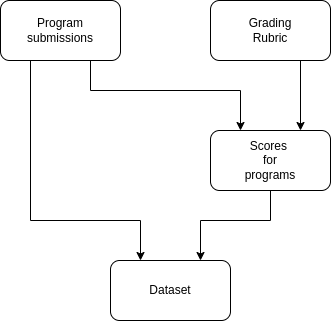
\includegraphics{./figures/data.png}
\caption{Data Annotation Flow}
\label{fig1}
\end{figure}

The score component for a value of 10 points was divided into
two parts namely \textbf{Design} (5 points) and
\textbf{Functionality} (5 points). The subsequent pattern
managed to cover the entirety of a code solution to provide a
value balancing the code's design and functionality.


For design, considering each problem has its own set of
parameters to satisfy, the grading rubric is adjusted based
on this requirement. The parameters used for evaluating
design is mentioned in Table~3.2. Tables~3.3 to 3.6 details
the appropriate score to respective problems based on their
necessary individual criteria for each different task.
        
        
\begin{table}[H]
\centering
\caption{Grading Parameters}
\begin{tabular}{|c|}
\hline
\emph{Parameters} \\ \hline
Use of Variables \\ \hline
Modularity \\ \hline
Logic Application \\ \hline
Efficiency \\ \hline
\end{tabular}

\label{tab:params}
\end{table}


\begin{itemize}
\item \textbf{Selection Sort}
  \begin{table}[h]
    \centering
    \caption{Grading Rubric (Design) for Selection Sort}
    \begin{tabular}{|l|c|}
      \hline
      \emph{Parameter}                                                          & \multicolumn{1}{l|}{\textbf{Weightage}} \\ \hline
      \begin{tabular}[c]{@{}l@{}}Code \\ modularity\\ \end{tabular}                  & 1                                       \\ \hline
      \begin{tabular}[c]{@{}l@{}}Use of \\ variables\\ \end{tabular}              & 1                                       \\ \hline
      \begin{tabular}[c]{@{}l@{}}The logic \\ applied\\ \end{tabular}             & 1                                       \\ \hline
      \begin{tabular}[c]{@{}l@{}}Efficient use \\ of functions\\ \end{tabular} & 2                                       \\ \hline
    \end{tabular}

    \label{ss_rub_design}
  \end{table}

  For ``Selection Sort'' task, three functions had to be
  defined: one for swapping, another to find the smallest
  element of the list from a given index, and yet another
  function for sorting which will use the other two
  functions. Hence, the definition of functions and use of
  function calls becomes the important parameter for design
  consideration.

\item \textbf{First Negative Element in List}

  \begin{table}[h!]
    \centering
    \caption{Grading Rubric (Design) for First Negative
      Element in List}
    \begin{tabular}{|l|c|}
      \hline
      \textbf{Parameter}                                                 & \multicolumn{1}{l|}{\textbf{Weightage}} \\ \hline
      \begin{tabular}[c]{@{}l@{}}Use of \\ variables\end{tabular}     & 1                                       \\ \hline
      \begin{tabular}[c]{@{}l@{}}The logic \\ applied\end{tabular}    & 2                                       \\ \hline
      \begin{tabular}[c]{@{}l@{}}Efficiency\\ of solution\end{tabular} & 2                                       \\ \hline
    \end{tabular}

    \label{fn_rub_design}
  \end{table}

  For ``First Negative Element in List'' task, there was no
  need of functions as it only requires a simple looping
  statement and a conditional statement to find the first
  negative element in the list. The important design
  parameter now was the logic applied to find the first
  negative element and the efficiency of the solution (for
  instance, the use of break statement after finding the
  first negative element).

\item \textbf{Largest Element in the List}

  \begin{table}[h!]
    \centering
    \caption{Grading Rubric (Design) for Largest Element in
      List task}
    \begin{tabular}{|l|c|}
      \hline
      \textbf{Parameter}                                                 & \multicolumn{1}{l|}{\textbf{Weightage}} \\ \hline
      \begin{tabular}[c]{@{}l@{}}Use of \\ variables\end{tabular}     & 2                                       \\ \hline
      \begin{tabular}[c]{@{}l@{}}The logic \\ applied\end{tabular}    & 1                                       \\ \hline
      \begin{tabular}[c]{@{}l@{}}Efficiency\\ of solution\end{tabular} & 2                                       \\ \hline
    \end{tabular}

    \label{la_rub_design}
  \end{table}

  For ``Largest Element in the List'' task, there was no need
  of functions again as it only requires a simple looping
  statement and a conditional statement to find and print the
  index of the largest element in the list. Here, the
  definition and use of variables was the important parameter
  along with the efficiency.

\item \textbf{Unique Character Count in String}

  \begin{table}[h!]
    \centering
    \caption{Grading Rubric (Design) for Unique Character
      Count in string}
    \begin{tabular}{|l|c|}
      \hline
      \textbf{Parameter}                                                 & \multicolumn{1}{l|}{\textbf{Weightage}} \\ \hline
      \begin{tabular}[c]{@{}l@{}}Use of \\ variables\end{tabular}     & 1                                       \\ \hline
      \begin{tabular}[c]{@{}l@{}}The logic \\ applied\end{tabular}    & 1                                       \\ \hline
      \begin{tabular}[c]{@{}l@{}}Code\\ Modularity\end{tabular}          & 1                                       \\ \hline
      \begin{tabular}[c]{@{}l@{}}Efficiency\\ of solution\end{tabular} & 2                                       \\ \hline
    \end{tabular}

    \label{uc_rub_design}
  \end{table}

  For ``Unique Character Count in String'' task, functions
  can be defined to check and ignore special characters, a
  function could be defined to count the unique tokens,
  etc. Thus, the code could be made modular.  Since this
  particular task could be solved in a variety of ways, the
  efficiency of the solution matters more.
\end{itemize}

% \begin{table}
% \centering
% \caption{Grading Rubric}
% \label{tab:rubric}
% \resizebox{\textwidth}{!}{%
% \begin{tabular}{|l|c|c|c|c|} 
% \cline{2-5}
% \multicolumn{1}{l|}{}                  & \multicolumn{4}{c|}{\begin{tabular}[c]{@{}c@{}}\textbf{}\\\textbf{Parameters}\\\textbf{}\end{tabular}}                                                                                                                                          \\ 
% \hline
% \multicolumn{1}{|c|}{\textbf{Program}} & \textit{\textbf{~ ~Use of Variables~~}} & \textit{\textbf{~ ~ Modularity~ ~~}} & \textit{\textbf{~ ~Logic application~~}} & \begin{tabular}[c]{@{}c@{}}\textit{\textbf{}}\\\textit{\textbf{~ ~Efficiency~ ~}}\\\textit{\textbf{}}\end{tabular}  \\ 
% \hline
% First Negative Element in List~ ~ ~ ~~ & 1                                       & -                                    & 2                                        & \begin{tabular}[c]{@{}c@{}}\\2\\\end{tabular}                                                                       \\ 
% \hline
% Selection Sort                         & 1                                       & 1                                    & 1                                        & \begin{tabular}[c]{@{}c@{}}\\2\\\end{tabular}                                                                       \\ 
% \hline
% Largest Element in List                & 1                                       & -                                    & 2                                        & \begin{tabular}[c]{@{}c@{}}\\2\\\end{tabular}                                                                       \\ 
% \hline
% Unique Count of Characters             & 1                                       & 1                                    & 1                                        & \begin{tabular}[c]{@{}c@{}}\\2\\\end{tabular}                                                                       \\
% \hline
% \end{tabular}%
% }
% \end{table}



% \begin{table}[h]
% \centering
% \label{tab:rubric}
% \resizebox{\textwidth}{!}{%
% \begin{tabular}{l|cccc|}
% \cline{2-5}
%  & \multicolumn{4}{c|}{\textbf{Parameters}} \\ \hline
% \multicolumn{1}{|c|}{\textbf{Program}} & \multicolumn{1}{l|}{\textit{\textbf{Use of Variables}}} & \multicolumn{1}{l|}{\textit{\textbf{Modularity}}} & \multicolumn{1}{l|}{\textit{\textbf{Logic application}}} & \multicolumn{1}{l|}{\textit{\textbf{Efficiency}}} \\ \hline
% \multicolumn{1}{|l|}{First Negative Element in List} & \multicolumn{1}{c|}{1} & \multicolumn{1}{c|}{-} & \multicolumn{1}{c|}{2} & 2 \\ \hline
% \multicolumn{1}{|l|}{Bank Account} & \multicolumn{1}{c|}{2} & \multicolumn{1}{c|}{1} & \multicolumn{1}{c|}{1} & 1 \\ \hline
% \multicolumn{1}{|l|}{Selection Sort} & \multicolumn{1}{c|}{1} & \multicolumn{1}{c|}{1} & \multicolumn{1}{c|}{1} & 2 \\ \hline
% \multicolumn{1}{|l|}{Largest Element in List} & \multicolumn{1}{c|}{1} & \multicolumn{1}{c|}{-} & \multicolumn{1}{c|}{2} & 2 \\ \hline
% \multicolumn{1}{|l|}{Unique Count of Characters} & \multicolumn{1}{c|}{1} & \multicolumn{1}{c|}{1} & \multicolumn{1}{c|}{1} & 2 \\ \hline
% \end{tabular}%
% }
% \caption{Grading Rubric}
% \end{table}

\newpage

For \textbf{functionality}, the following rubric mentioned in
Table~3.7 was followed to give a score in a scale of 5. The
correctness and completeness of the code was considered to
grade the code submissions.

\begin{table}[H]
\centering
\caption{Grading Rubric (Functionality)}
\begin{tabular}{|l|c|}
\hline
\textbf{\begin{tabular}[c]{@{}l@{}}Code's correctness\\ and \\ completeness\end{tabular}} & \multicolumn{1}{l|}{\textbf{Score}} \\ \hline
\begin{tabular}[c]{@{}l@{}}Perfectly correct\\ and complete\end{tabular}                     & 5                                   \\ \hline
\begin{tabular}[c]{@{}l@{}}Correct and complete\\ but can be improved\end{tabular}           & 4                                   \\ \hline
\begin{tabular}[c]{@{}l@{}}Complete but \\ partially incorrect\end{tabular}                  & 3                                   \\ \hline
\begin{tabular}[c]{@{}l@{}}Incomplete and\\ partially correct\end{tabular}                   & 2                                   \\ \hline
\begin{tabular}[c]{@{}l@{}}Incomplete and\\ totally incorrect\end{tabular}                   & 1                                   \\ \hline
\end{tabular}

\label{grading_rub}
\end{table}

Finally, a dataset compiled of code solutions and appropriate
numeric score values (in the range from 0 to 10) was
generated to be used for the subsequent experimentation.

\newpage

\subsection{Example Code Submissions}

Figures~3.2 to 3.9 document the examples of best and worst
programs for each problem with scores assigned using the
developed grading rubric.

\subsubsection{Selection Sort}

\begin{figure}[h]
\centering
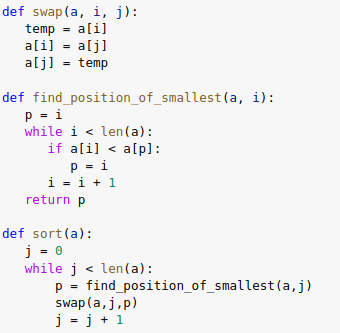
\includegraphics[]{./figures/best_ss.png}
\caption{Best Program - Selection Sort}
\label{fig1}
\end{figure}

\begin{figure}[H]
\centering
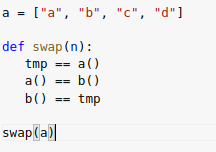
\includegraphics[scale=1.2]{./figures/ss_worst.png}
\caption{Worst Program - Selection Sort}
\label{fig1}
\end{figure}


Figures 3.2 is one of the best program submissions for the
selection sort task. The program was properly structured with
three functions, one to do swapping, one to find smallest
element's position from a given index from the list, and
finally the sort function which will utilise the first two
functions inside a loop to sort the list. Hence, it was
awarded a perfect 10/10.

Figure 3.3 is one of the worst program submissions. This code
solution has a swap function defined but with wrong logic. A
unnecessary global variable 'a' was declared. The logic of
the swap function was not right. Hence this solution was
graded 1/10.

\newpage
\subsubsection{First negative element in a list}

\begin{figure}[h]
\centering
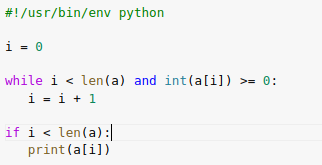
\includegraphics{./figures/best_fn.png}
\caption{Best Program - First negative element in a list}
\label{fig1}
\end{figure}

\begin{figure}[h]
\centering
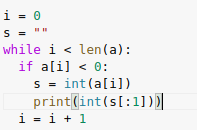
\includegraphics{./figures/worst_fn.png}
\caption{Worst Program - First negative element in a list}
\label{fig1}
\end{figure}

Figure~3.4 shows a good solution for finding the first
negative element in the list. The loop traverses the list
until it finds the first negative element. When that index
belongs to the list, the program prints the first negative
element. The program is graded a perfect 10/10.

Figure~3.5 shows one of the bad code solutions submitted. The
program is graded only 3/10 for using wrong logic and also
for improper declaration and use of variables.

\newpage

\subsubsection{Unique characters count in a string}

\begin{figure}[h]
\centering
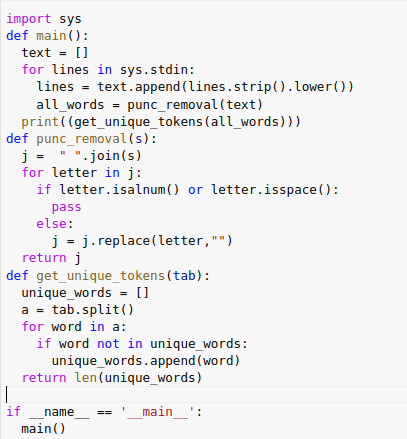
\includegraphics{./figures/best_uc.png}
\caption{Best Program - Unique characters count in a string}
\label{fig1}
\end{figure}

\newpage

\begin{figure}[H]
\centering
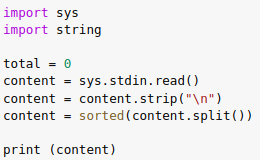
\includegraphics{./figures/worst_uc.png}
\caption{Worst Program - Unique characters count in a string}
\label{fig1}
\end{figure}

Figure 3.6 is one of the best program submissions for the
unique character count task. The code is properly organised,
modular with three functions and the code has perfect
logic. No unnecessary global variable is defined. Thus, this
particular submission was awarded with the perfect score of
10.

Figure 3.7 on the other hand shows one of the worst
submissions for this particular task. No functions have been
defined. An unnecessary global variable was declared. The
code would not yield the expected result. Thus, this code was
only given a score of 1.

\newpage

\subsubsection{Largest element of a list}

\begin{figure}[h]
\centering
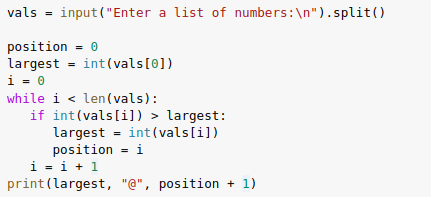
\includegraphics{./figures/best_la.png}
\caption{Best Program - Largest element of a list}
\label{fig1}
\end{figure}

\begin{figure}[h]
\centering
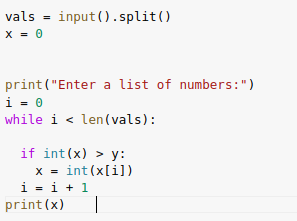
\includegraphics{./figures/worst_la.png}
\caption{Worst Program - Largest element of a list}
\label{fig1}
\end{figure}

\newpage

Figure 3.8 is one of the best student code submissions for
the largest element task. This particular solution has the
right logic.  Variables have been used properly. The program
prints the correct position of the largest element in the
list. Looping and conditional statements have been used
correctly. Thus, this solution was awarded as score of 10.

Figure 3.9 is one of the worst student submissions for this
task. Variables have not been properly used. The logic used
is also wrong. Hence, this code solution was only given a
score of 2.

\newpage

\section{FEATURE EXTRACTION}

Following the annotation of the dataset, feature extraction
and feature selection are performed for optimal
representation of code solutions as vectors for
regression. The following series of steps were performed for
extracting meaningful features from the dataset.

\begin{itemize}
\item \textbf{Py2 to Py3 conversion}: The code solutions in
  the dataset are documented in Python 2 version. To support
  extraction of features, Python 2 to Python 3 conversion was
  performed using the '2to3' module \cite{G}.
\item \textbf{Abstract Syntax Tree (AST) representation}:
  After converting every program to Python 3 format, the AST
  \cite{F} representation for each program was computed to
  derive appropriate features. The inbuilt Python `ast'
  module was used to get the ast representation of the
  student submissions. The `ast' module provides a `parse()'
  method which returns the AST representation of a program. A
  variety of features can be extracted from this ast
  representation with the help of `walk()' function provided
  by the `ast' module. The extracted features from the AST
  representation are documented in Table~3.9. Other features
  derived from code are represented in Table~3.8.
\end{itemize}

\begin{table}[H]
\centering
\caption{Features extracted from code}
\begin{tabular}{|l|l|} 
\hline
return       & Count of 'return' statements in the code      \\ 
\hline
break        & Count of 'break' statements in the code       \\ 
\hline
continue     & Count of 'continue' statements in the code    \\ 
\hline
pass         & Count of 'pass' statements in the code        \\ 
\hline
assign       & Count of assignment operators in the code     \\ 
\hline
arith        & Count of arithmetic operators in the code     \\ 
\hline
comp         & Count of comparison operators in the code     \\ 
\hline
log          & Count of logical operators in the code        \\ 
\hline
cond         & Count of conditional operators in the code    \\ 
\hline
loop         & Count of 'for' and 'while' loops in the code  \\ 
\hline
\#lines      & Count of lines in the code                    \\ 
\hline
\end{tabular}
\end{table}

\begin{table}[H]
\centering
\caption{Features extracted from AST} 
\begin{tabular}{|l|l|} 
\hline 
\#fun                 & Count of function definitions in the code                                                                                      \\ 
\hline
\#fcall               & Count of function calls in the code                                                                                            \\ 
\hline
globals               & Count of globals variables in the code                                                                                         \\ 
\hline
\#lst                 & Count of lists and tuples in the code                                                                                          \\ 
\hline
\#var                 & \begin{tabular}[c]{@{}l@{}}Count of the variables in the code\\(Count of variables defined)\end{tabular}                       \\ 
\hline
\#var\_uses           & \begin{tabular}[c]{@{}l@{}}Count of variable uses in the code\\(Count of variables used in different statements)\end{tabular}  \\ 
\hline
\end{tabular}
\end{table}


Ultimately we extracted 17 features(11 from source code and 6 from AST representation of source code).

\newpage
\section{FEATURE SELECTION}

After extracting meaningful features from both the code and
AST representation (Table~3.8, Table~3.9), feature
selection is performed for each problem considering feature
sets for each problem are independent of each other and are
problem dependent.

Firstly, the features that share the same value for all the
code solutions are identified and removed to avoid
redundancy. Once the redundant features are reduced, the
number of features eventually reduces from
\begin{itemize}
\item 17 to 14 for 'Selection sort'
\item 17 to 12 for 'The First negative element in the list'
\item 17 to 12 for 'The Largest Element in List'
\item 17 to 15 for 'The unique character count in a string
  task.'
\end{itemize}
Then, the best features are selected for each task according
to how well they are correlated with the target variable. The
\emph{f\_regression} method \cite{H} returns the degree of
correlation (F-statistic) between each feature and the
target.

The correlation F-statistic score of different features for
the tasks are listed as tables below. After the F-statistic
score is calculated, the features which have significant
influence on the target variable(score) are selected and the
regressor model for each task is trained with the selected
features.

\subsection{Implementation}

Tables~3.10 to 3.14 report the F-Statistic score of the
features set with their respective scores. The strike-through
text in features list of the tables represent the features
that are dropped due to their low $f{reg}$ score.

\begin{itemize}
\item \textbf{Selection Sort}
  \begin{table}[H]
    \centering
    \caption{F-statistic table : Selection Sort}
    \begin{tabular}{|l|l|}
      \hline
      \textbf{Feature} & \textbf{$f{reg}$ score} \\ \hline
      \#fun            & 387.16                \\ \hline
      loop             & 181.29                \\ \hline
      \#fcall          & 179.15                \\ \hline
      \#var\_uses      & 122.33                \\ \hline
      comp             & 104.35                \\ \hline
      \#lines          & 91.83                 \\ \hline
      return           & 91.55                 \\ \hline
      arith            & 68.54                 \\ \hline
      assign           & 65.93                 \\ \hline
      \#var            & 56.68                 \\ \hline
      cond             & 50.10                 \\ \hline
      \#lst            & 20.39                 \\ \hline
      globals          & 15.75                 \\ \hline
      \st{log}              & 1.81                  \\ \hline
    \end{tabular}
            
    \label{ss_f}
  \end{table}
            
  From Table 3.10, it can be observed that for 'Selection
  sort' task, the number of functions, loops, function calls,
  variable uses and comparison operators have a very strong
  correlation with the output score. The first 13 features
  have a considerably big influence on the target variable
  when compared to that of number of logical operators.
            
\item \textbf{First Negative Element in List}

  \begin{table}[H]
    \centering
    \caption{F-statistic table : First Negative Element in
      List}
    \begin{tabular}{|l|l|}
      \hline
      \textbf{Feature} & \textbf{$f{reg}$ score} \\ \hline
      comp             & 31.42                 \\ \hline
      \#var\_uses      & 6.33                  \\ \hline
      cond             & 6.02                  \\ \hline
      log              & 2.11                  \\ \hline
      assign           & 2.02                  \\ \hline
      loop             & 1.85                  \\ \hline
      break            & 1.49                  \\ \hline
      \#lines          & 1.47                  \\ \hline
      \#var            & 1.32                  \\ \hline
      \#lst            & 1.01                  \\ \hline
      \st{globals}          & 0.50                  \\ \hline
      \st{arith}            & 0.05                  \\ \hline

    \end{tabular}

    \label{fn_f}
  \end{table}

  From Table 3.11, it is observed that for the 'First
  negative element in the list' task, the number of
  comparison statements have a large correlation on the
  output variable. The number of variable uses and the number
  of conditional statements also have a good influence with
  the target variable. Here with a minimum cutoff of a F-reg
  score of 1, top 10 features become the selected features.

\newpage

\item \textbf{Largest Element in List}

\begin{table}[H]
\centering
\caption{F-statistic table : Largest Element in List}
\begin{tabular}{|l|l|}
\hline
\textbf{Feature} & \textbf{$f{reg}$ score} \\ \hline
assign           & 17.51                 \\ \hline
arith            & 15.91                 \\ \hline
\#var\_uses      & 12.47                 \\ \hline
globals          & 9.47                  \\ \hline
\#lst            & 3.82                  \\ \hline
comp             & 3.35                  \\ \hline
cond             & 3.35                  \\ \hline
\#var            & 2.49                  \\ \hline
\st{loop}             & 0.90                  \\ \hline
\st{break}            & 0.84                  \\ \hline
\st{\#lines}          & 0.73                  \\ \hline
\st{log}              & 0.02                  \\ \hline

\end{tabular}

\label{la_f}
\end{table}

From Table 3.12, it is observed for the 'Largest element in
the list' task, the number of assignment statements,
arithmetic operators and variable uses have a great influence
on the final target value. With a minimum cutoff of a F-reg
score 1.0 the top 8 features are selected.

\newpage

\item \textbf{Unique Character Count in List}

\begin{table}[H]
\centering
\caption{F-statistic table : Unique Character Count in List}
\begin{tabular}{ll}
\hline
\multicolumn{1}{|l|}{\textbf{Feature}} & \multicolumn{1}{l|}{\textbf{$f{reg}$ score}} \\ \hline
\multicolumn{1}{|l|}{log}              & \multicolumn{1}{l|}{15.76}                 \\ \hline
\multicolumn{1}{|l|}{\#fcall}          & \multicolumn{1}{l|}{4.94}                  \\ \hline
\multicolumn{1}{|l|}{\#var}            & \multicolumn{1}{l|}{3.58}                  \\ \hline
\multicolumn{1}{|l|}{cond}             & \multicolumn{1}{l|}{3.52}                  \\ \hline
\multicolumn{1}{|l|}{pass}             & \multicolumn{1}{l|}{3.42}                  \\ \hline
\multicolumn{1}{|l|}{\#var\_uses}      & \multicolumn{1}{l|}{3.22}                  \\ \hline
\multicolumn{1}{|l|}{\#lst}            & \multicolumn{1}{l|}{2.91}                  \\ \hline
\multicolumn{1}{|l|}{loop}             & \multicolumn{1}{l|}{1.91}                  \\ \hline
\multicolumn{1}{|l|}{\st{return}}           & \multicolumn{1}{l|}{0.95}                  \\ \hline
\multicolumn{1}{|l|}{\st{comp}}             & \multicolumn{1}{l|}{0.78}                  \\ \hline
\multicolumn{1}{|l|}{\st{\#fun}}            & \multicolumn{1}{l|}{0.46}                  \\ \hline
\multicolumn{1}{|l|}{\st{\#lines}}          & \multicolumn{1}{l|}{0.34}                  \\ \hline
\multicolumn{1}{|l|}{\st{globals}}         & \multicolumn{1}{l|}{0.20}                  \\ \hline
\multicolumn{1}{|l|}{\st{arith}}            & \multicolumn{1}{l|}{0.17}                  \\ \hline
\multicolumn{1}{|l|}{\st{assign}}           & \multicolumn{1}{l|}{0.05}      
\\ \hline
\end{tabular}

\label{uc_f}
\end{table}

From Table 3.13, it is observed for the unique character
count in a string, the number of logical operators has the
highest influence on the final target output. This is due to
the number of 'not' and 'not in' operators. With a minimum
cutoff set at a F-reg score of 1.0, only the first eight
features are selected.
\end{itemize} % IMPLEMENTATION
% Chapter 3

\chapter{DESIGN AND ARCHITECTURE}

% \begin{figure}[hbt] 
% \begin{center}
% \includegraphics[scale=.40]{./figures/bddig1}
% \caption{\label{fig:BDDD}A BDD where some boolean variables occur more than
% once on an evaluation path.}
% \end{center}
% \end{figure}

We propose a machine learning based student program evaluation system which represents student programs as a set of features extracted from the source programs and the AST representation of the source programs. Deep learning is purposely avoided since it would make the program's representation difficult to comprehend. The ML models are regression models which will output a score between 0 to 10 for each program submission. Feedback is provided to each program submission based on comparing the feature vector of the program with the average feature vector of 'good' programs.


\section{TRAINING} 

The dataset contains the code and corresponding scores for each of the
student programs. Features from code were extracted by using two
ways. Some features were extracted directly from the code. For the
other features, the code was first transformed into an Abstract Syntax
Tree(AST); then the features were extracted from the AST. The extracted
features were used to train the model. Three models were trained
separately: Linear Support vector regressor(SVR) , Random forest and Multi layer
perceptron(MLP) regressor. The models trained were all regression models which were
trained to predict the scores that should be given to the evaluated
codes.

\begin{figure}[h]
\centering
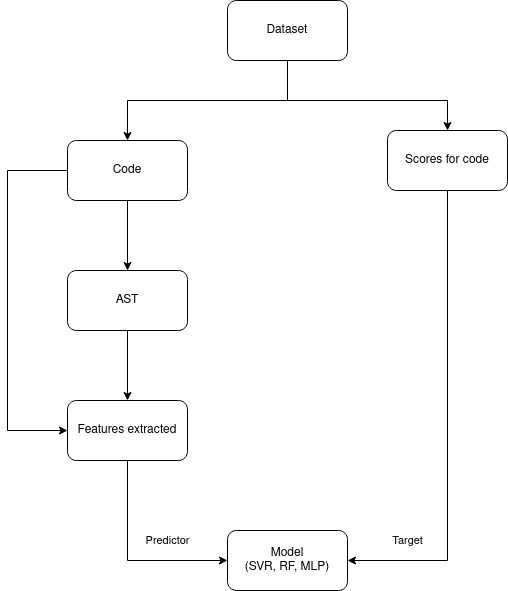
\includegraphics[width=0.9\textwidth]{./training.jpg}
\caption{Training}
\label{fig1}
\end{figure}

\newpage

\section{DEPLOYMENT} 

\begin{figure}[H]
\centering
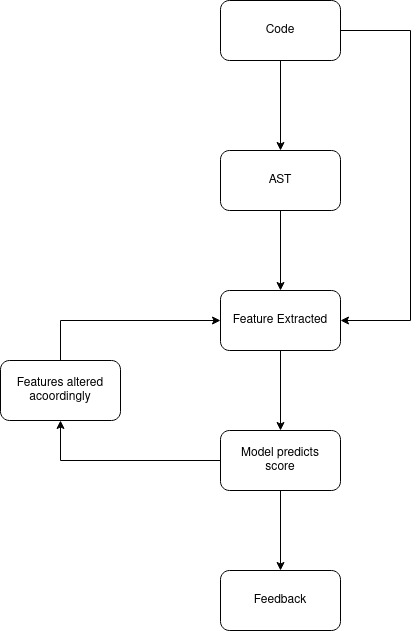
\includegraphics[scale=0.7]{./Deployment.jpg}
\caption{Deployment}
\label{fig1}
\end{figure}

The student code is the input. Features are extracted from the code as
explained in the section above. Some features are extracted from the
code itself and the rest from an AST representation of the code. This
feature set is input into the trained models from the previous
section. The model predicts a score for the input code based on the
feature set.

As explained earlier, our model is trained only with the feature values of the program and its score. Our trained model will evaluate how modifications in program's features can lead to a better score and thus there is no necessity for a explicitly annotated dataset with feedbacks for each code. 

From the training dataset, average feature vector $x$ is computed for the "excellent" programs(programs with a perfect score of 10). Feedback is generated with correspondence to the difference between the feature values of the submitted program and the average feature vector of the excellent programs.



\section{ALGORITHMS}

After representing code solutions as feature vectors, the dataset was
exported to perform training for machine learning models. The
following models
\begin{itemize}
    \item Support Vector Machine (SVM)
    \item Random Forest 
    \item Multi Layer Perceptron (MLP)
\end{itemize}
were employed for training. The detailed description of the mentioned
algorithms are listed below.

\section{SUPPORT VECTOR MACHINE}

Support Vector Machines (SVMs) are supervised learning models with associated learning algorithms that examine data for classification and regression in machine learning. Support Vector Regression \cite{D} is used to predict continuous values. The Support Vector Machine and Support Vector Regression are both based on the same premise (SVM). The goal of a support vector machine method is to find a hyperplane in an n-dimensional space that categorises data points clearly. Support Vectors are the data points on each side of the hyperplane that are closest to the hyperplane. These have an effect on the hyperplane's location and orientation, and so aid in the construction of the SVM.

\subsection{Hyperparameters in SVR}

Following are the various key hyper parameters used in Support Vector Regression.
\begin{figure}[h]
\centering
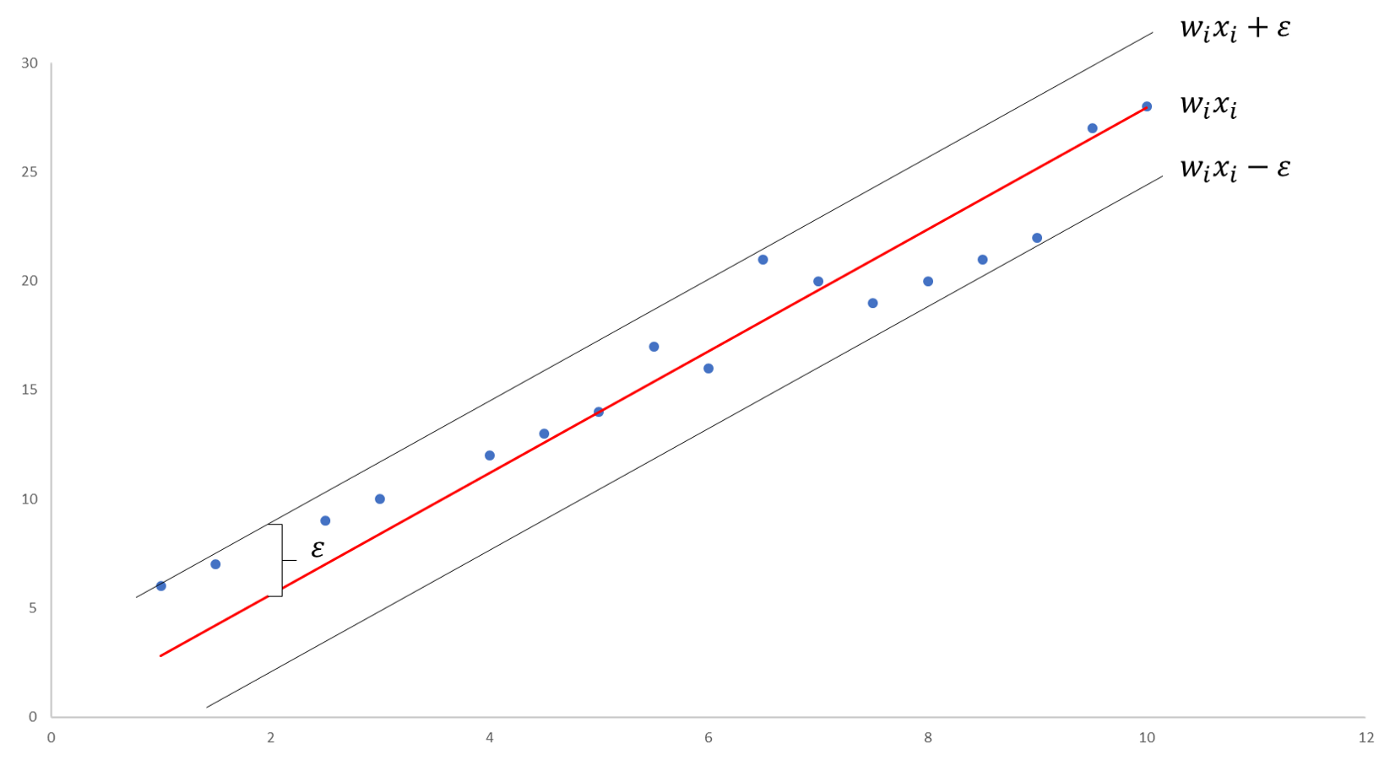
\includegraphics[width=1\textwidth, height=15cm]{./figures/svm.png}
\caption{Simple SVR}
\label{fig1}
\end{figure}

\begin{itemize}
\item \textbf{Hyperplane} (Red line in Figure~4.3) \\ A decision boundary that forecasts continuous output is known as a hyperplane. Support Vectors are the data points on each side of the hyperplane that are closest to the hyperplane. These are used to draw the essential line that depicts the algorithm's projected outcome.
\item \textbf{Kernel} \\ A kernel is a collection of mathematical functions that take input data and transform it into the required form. These are most commonly employed to locate a hyperplane in higher-dimensional space.
\item \textbf{Boundary Lines} (Grey lines in Figure~4.3) \\ 
These are the two lines that are drawn at an \textbf{$\epsilon$} (epsilon) distance around the hyperplane. It's used to separate the data points by a margin.

\end{itemize}

\subsection{Support Vector Regression}

The best fit line or hyperplane with the most points is found using Support Vector Regression (SVR). The SVR, unlike other regression models, aims to fit the best line within a threshold value, rather than minimising the error between the real and projected value (the distance between the hyperplane and boundary line). As a result, we'll only consider points that fall inside the decision boundary and have the lowest error rate, or those that fall within the margin of tolerance. This results in a more accurate model.

%\newpage

\section{RANDOM FOREST}

Random forest is a frequently used supervised machine learning algorithm for classification and regression tasks. The functioning of
Random Forest is contingent on three main factors,
\begin{itemize}
\item Decision Trees
\item Ensemble Learning
\item Bootstrapping
\end{itemize}

The following subsections % (6.2.1, 6.2.2 and 6.2.3)
detail on the mentioned factors description.

\subsection{Ensemble Learning}

Ensemble learning is the process of combining many models that have been trained on the same data and averaging their findings to provide a more accurate predictive/classification result. Ensemble learning requires that the errors of each model (a decision tree model) be independent and distinct from one another.

\subsection{Decision Tree}

\begin{figure}[h]
\centering
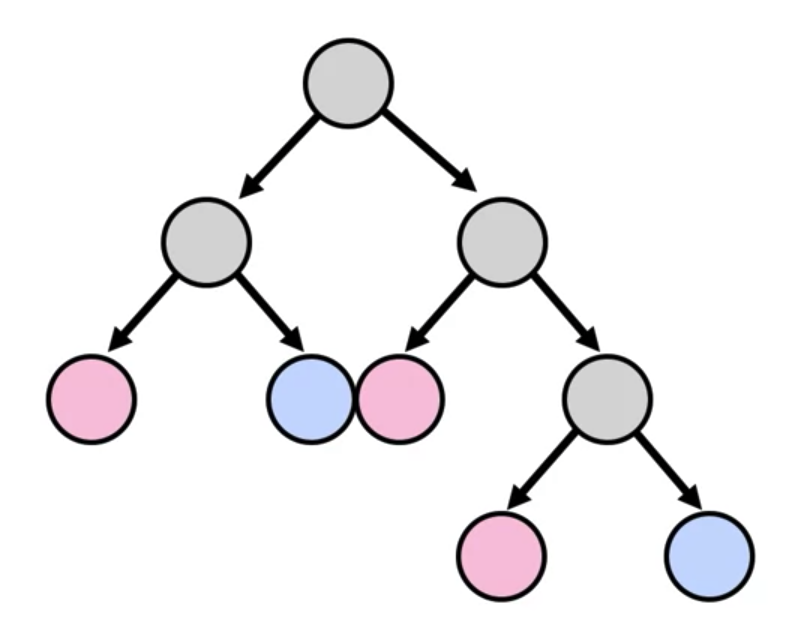
\includegraphics[scale=.5]{./figures/dectree.png}
\caption{Decision tree layout}
\label{fig1}
\end{figure}

Both regression and classification issues can be solved using decision trees. The objective is to learn basic decision rules from data attributes to develop a model that predicts the value of a target variable. They begin at the root of the tree and go via splits depending on varied outcomes until they reach a leaf node where the result is delivered.Figure~4.4 details a visual representation of the decision
tree layout.

\subsection{Bootstrapping}

The process of randomly sampling subsets of a dataset across a specified number of repetitions and variables is known as bootstrapping. To get a more accurate result, these results are averaged together.

\subsection{Random Forest Regression}

\begin{figure}[H]
\centering
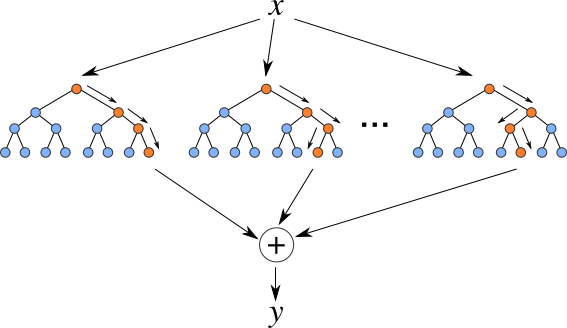
\includegraphics[width=1\textwidth, height=9cm]{./figures/rf.png}
\caption{Simple RF}
\label{fig1}
\end{figure}

The bootstrapping Random Forest algorithm \cite{B} combines ensemble learning techniques with the decision tree framework to generate numerous randomly drawn decision trees from data, then averaging the results to produce a new result that typically leads to better predictions/classifications. Figure~4.5 documents a visual
representation of random forest wherein $X$ is the feature
vector and $y$ is the target vector.

\section{MULTI LAYER PERCEPTRON}

The Multi Layer Perceptron bases its fundamental design to the
interlinking of several neuron-like structures representing a Neural
Network (NN) architecture. Given $i = 0,1,\ldots,n$ where $n$ is the
number of inputs, the quantities $w_{i}$ are the weights of the
neuron. The inputs $x_{i}$ correspond to features or variables and the
output $y$ to their prediction/estimation. Figure~4.6 shows the
simplified representation of the above steps.

\begin{figure}[h]
\centering
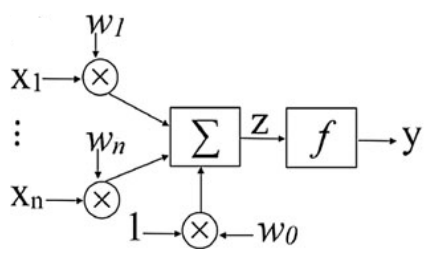
\includegraphics[]{./figures/perceptron.png}
\caption{Perceptron model}
\label{fig1}
\end{figure}

The weighting step involves the multiplication of each input feature
value by its weight ${w_ix_i}$ and then they are summed
together $(x_{0}w_{0} + x_{1}w_{1} + ... + x_{n}w_{n})$. In the transfer step, an activation function f (also called a
transfer function) is applied to the sum producing an output $y$
presented as
\begin{equation}
  z & = \sum_{i=0}^{n} w_{i}x_{i}\\
\end{equation}
\begin{equation}
  y & = f(z)
\end{equation}
wherein $x_{0} = 0$, $w_{0}$ is the bias and $y$ is the output. The
activation function can be of the form of Unit step, Linear or
Logistic operation.

For $n$
dimensions, the function is a hyperplane with equation:
\begin{equation}
    \sum_{i=0}^{n} w_{i}x_{i} = 0
\end{equation}

The goal of learning is to minimise a cost function, which is commonly a square error between the known and estimated vectors, in order to optimise the weights. The best weight vector can be determined using optimization techniques such as the gradient descent algorithm. The algorithm eventually converges on a solution that reaches an operational configuration network. The perceptron and single layer perceptron, on the other hand, do not address the nonlinearly separable problem.

\begin{figure}[h]
\centering
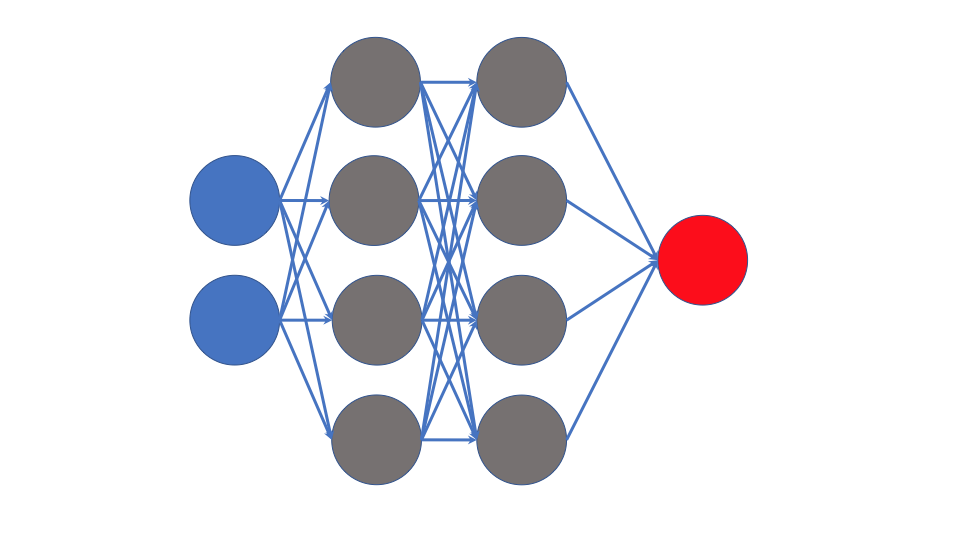
\includegraphics[width=1\textwidth]{./figures/mlp2.png}
\caption{MLP model}
\label{fig1}
\end{figure}

To solve this problem, Multi Layer Perceptron (MLP) architecture is
created by aggregating layers of perceptrons wherein the output of one
layer acts as the input of another layer. Multi Layer Perceptron
\cite{C} is a feedforward neural network that consists of three
layers, the input layer, the hidden layer and the output
layer. Figure~4.7 presents an MLP with two inputs (blue), two hidden
layers (grey) and one output (red).

The input signal to be processed is received by the input layer. The output layer is responsible for tasks such as prediction and categorization. The true computational engine of the MLP is an arbitrary number of hidden layers inserted between the input and output layers. In an MLP, data flows from input to output layer in the forward direction, similar to a feed forward network. The weights of the neurons in the MLP can be adjusted by propagating errors from layer to layer, starting with the output layer and going backwards, using the back propagation learning process. MLPs can tackle issues that aren't linearly separable and are designed to approximate any continuous function.
 % CONCLUSION AND FUTURE WORK
%% Chapter 5

\chapter{ALGORITHMS} % Write in your own chapter title

After representing code solutions as feature vectors, the dataset was exported to perform training for machine learning models. The following models 

\begin{itemize}
    \item Support Vector Machine (SVM)
    \item Random Forest 
    \item Multi Layer Perceptron (MLP)
\end{itemize}

were employed for training. The detailed description of the mentioned algorithms are listed below. 

\section{SUPPORT VECTOR MACHINE}

In machine learning, Support Vector Machines are supervised learning models with associated learning algorithms that analyze data used for classification and regression analysis. Support Vector Regression \cite{D} is a supervised learning algorithm that is used to predict discrete values. Support Vector Regression uses the same principle as the Support Vector Machine (SVM). The objective of a support vector machine algorithm is to find a hyperplane in an n-dimensional space that distinctly classifies the data points. The data points on either side of the hyperplane that are closest to the hyperplane are called Support Vectors. These influence the position and orientation of the hyperplane and thus help build the SVM.

\subsection{Hyperparameters in SVR}

Following are the various key hyper parameters used in Support Vector Regression.

\begin{figure}[h]
\centering
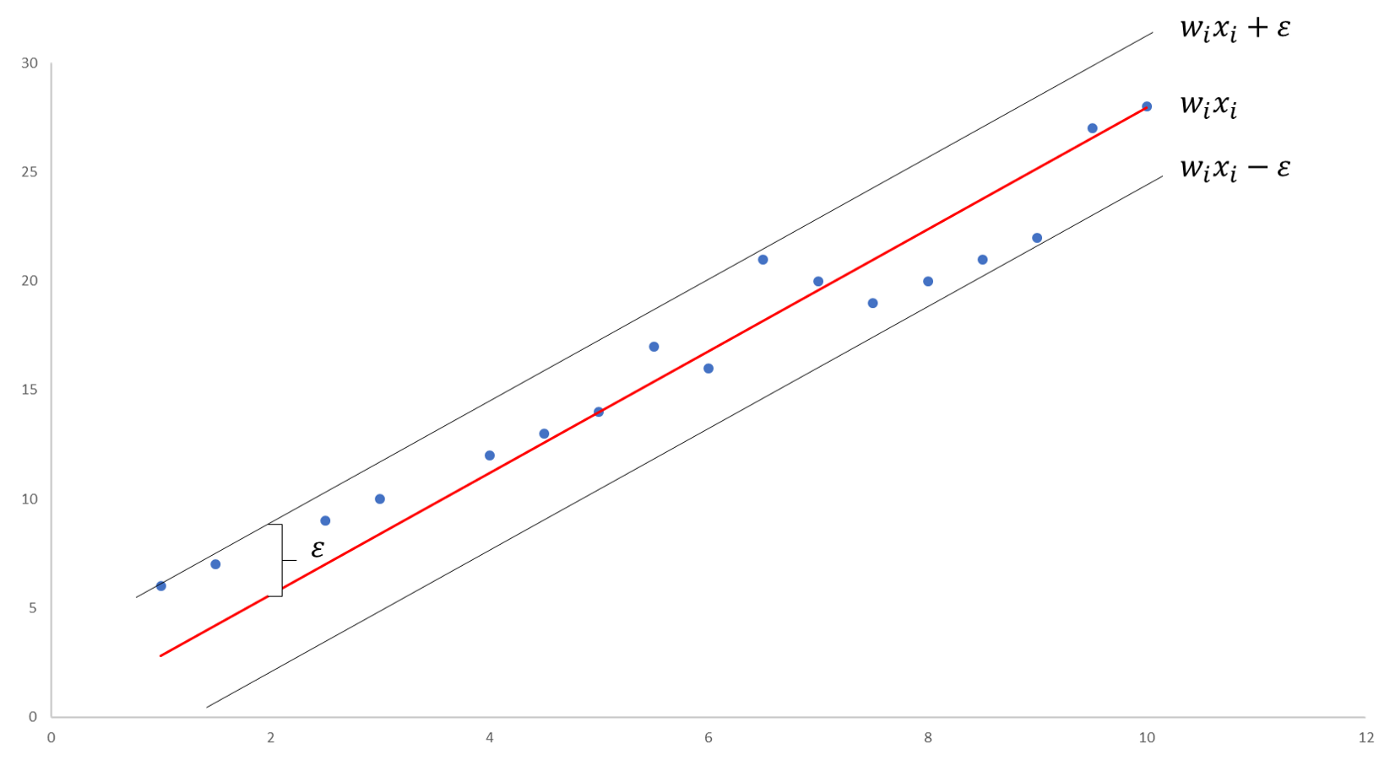
\includegraphics[width=1\textwidth, height=15cm]{./figures/svm.png}
\caption{Simple SVR}
\label{fig1}
\end{figure}

\begin{itemize}
    \item \textbf{Hyperplane} (Red line in Figure 6.1) \\ Hyperplanes are decision boundaries that is used to predict the continuous output. The data points on either side of the hyperplane that are closest to the hyperplane are called Support Vectors. These are used to plot the required line that shows the predicted output of the algorithm.
    \item \textbf{Kernel} \\ A kernel is a set of mathematical functions that takes data as input and transform it into the required form. These are generally used for finding a hyperplane in the higher dimensional space.
    \item \textbf{Boundary Lines} (Grey lines in Figure 6.1) \\ These are the two lines that are drawn around the hyperplane at a distance of \textbf{$\epsilon$} (epsilon). It is used to create a margin between the data points.
\end{itemize}

\subsection{Support Vector Regression}

Support Vector Regression (SVR) finds the best fit line or the hyperplane that has the maximum number of points. Unlike other Regression models that try to minimize the error between the real and predicted value, the SVR tries to fit the best line within a threshold value (the distance between the hyperplane and boundary line). 

Hence, we are going to take only those points that are within the decision boundary and have the least error rate, or are within the Margin of Tolerance. This gives us a better fitting model.

\newpage

\section{RANDOM FOREST}

Random forest is a Supervised Machine Learning Algorithm that is used widely in Classification and Regression problems. The functioning of Random Forest is contingent on three main factors, 

\begin{itemize}
    \item Decision Trees
    \item Ensemble Learning
    \item Bootstrapping
\end{itemize}

The following subsections (6.2.1, 6.2.2 and 6.2.3) detail on the mentioned factors description. 

\subsection{Ensemble Learning}

Ensemble learning is the process of using multiple models, trained over the same data, averaging the results of each model ultimately finding a more accurate predictive/classification result. The requirement for ensemble learning is that the errors of each model (in this case decision tree) are independent and different from tree to tree.

\subsection{Decision Tree}

\begin{figure}[h]
\centering
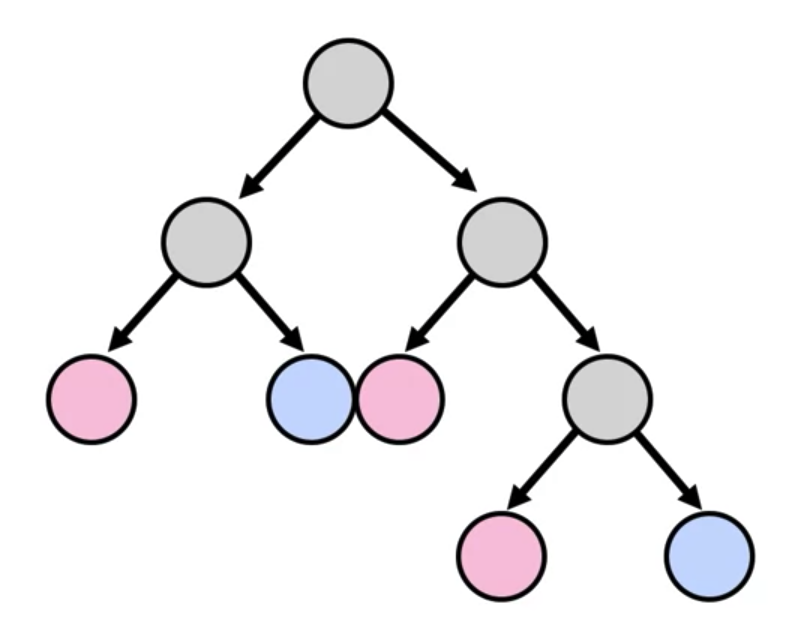
\includegraphics[width=1\textwidth]{./figures/dectree.png}
\caption{Decision tree layout}
\label{fig1}
\end{figure}

Decision Trees are used for both regression and classification problems. The goal is to create a model that predicts the value of a target variable by learning simple decision rules inferred from the data features. They start with the root of the tree and follow splits based on variable outcomes until a leaf node is reached and the result is given. Figure 6.2 details a visual representation of the decision tree layout. 

\subsection{Bootstrapping}

Bootstrapping is the process of randomly sampling subsets of a dataset over a given number of iterations and a given number of variables. These results are then averaged together to obtain a more accurate result. 

\subsection{Random Forest Regression}

\begin{figure}[h]
\centering
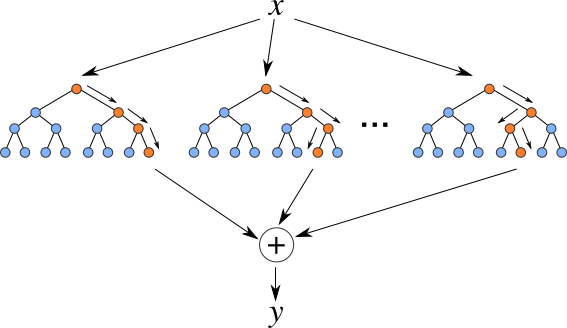
\includegraphics[width=1\textwidth, height=12cm]{./figures/rf.png}
\caption{Simple RF}
\label{fig1}
\end{figure}

The bootstrapping Random Forest algorithm \cite{B} combines ensemble learning methods with the decision tree framework to create multiple randomly drawn decision trees from the data, averaging the results to output a new result that often leads to strong predictions/classifications. Figure 6.2 documents a visual representation of random forest wherein \textbf{X} is the feature vector and \textbf{y} is the target vector. 

\section{MULTI LAYER PERCEPTRON}

The Multi Layer Perceptron bases its fundamental design to the interlinking of several neurons (like structures) representing a Neural Network (NN) architecture. Given $i = 0,1,..,n$ where n in the number of inputs, the quantities $w_{i}$ are the weights of the neuron. The inputs $x_{i}$ correspond to features or variables and the output y to their prediction/estimation. Figure 6.4 shows the simplified representation of the above steps.  

\begin{figure}[h]
\centering
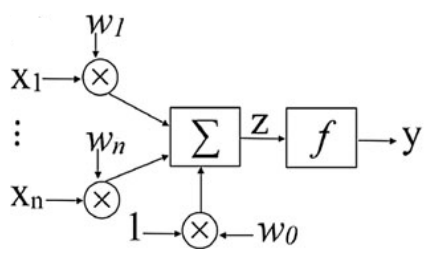
\includegraphics[]{./figures/perceptron.png}
\caption{Perceptron model}
\label{fig1}
\end{figure}

The weighting step involves the multiplication of each input feature value by its weight ${xiwi}$ and in the second step they are added together $(x_{0}w_{0} + x_{1}w_{1} + ... + x_{n}w_{n})$. The third is the transfer step where an activation function f (also called a transfer function) is applied to the sum producing an output y presented as:

\begin{equation}
    y = f(z)\;and\;z = \sum_{i=0}^{n} w_{i}x_{i}
\end{equation}

wherein $x_{0} = 0$, $w_{0}$ is the bias and y is the output. The activation function can be of the form of Unit step, Linear or Logistic operation. 

A perceptron can only learn linearly separable functions. For n dimensions, the function is a hyperplane with equation:

\begin{equation}
    \sum_{i=0}^{n} w_{i}x_{i} = 0
\end{equation}

The motive of learning is to optimize the weights by minimizing a cost function, which is usually a square error between the known vector and the estimated vector. Optimization techniques such as gradient descent algorithm can be used to determine the optimum weight vector. Ultimately, the algorithm converges to a solution reaching an operational configuration network. However, the perceptron and the single layer perceptron do not resolve the nonlinearly separable problem. 

\begin{figure}[h]
\centering
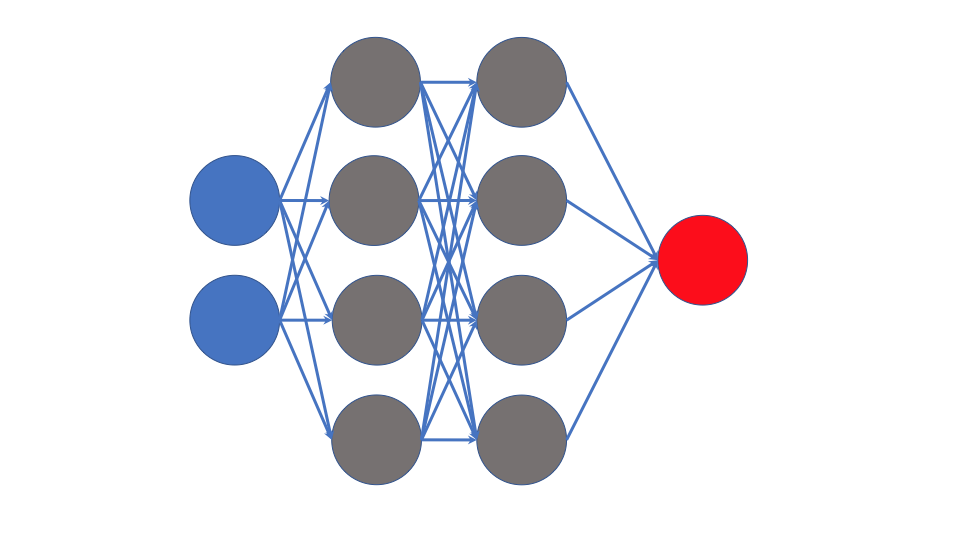
\includegraphics[width=1\textwidth]{./figures/mlp2.png}
\caption{MLP model}
\label{fig1}
\end{figure}

To solve this problem, Multi Layer Perceptron (MLP) architecture is created by aggregating layers of perceptrons wherein the output of one layer acts as the input of another layer. Multi Layer Perceptron \cite{C} is a feedforward neural network that consists of three layers, the input layer, the hidden layer and the output layer. Figure 6.5 presents an MLP with two inputs (blue), two hidden layers (grey) and one output (red). 

The input layer receives the input signal to be processed. The required task such as prediction and classification is performed by the output layer. An arbitrary number of hidden layers that are placed in between the input and output layer are the true computational engine of the MLP. Similar to a feed forward network in a MLP the data flows in the forward direction from input to output layer. The neurons in the MLP are trained with the back propagation learning algorithm, where the weights can be corrected by propagating the errors from layer to layer starting with the output layer and working backwards. MLPs are designed to approximate any continuous function and can solve problems which are not linearly separable.





\chapter{IMPLEMENTATION}

The implementation of models mentioned in Chapter 6 was performed
using the Scikit-Learn library \cite{E}. For each code submission
task, the dataset was split in the ratio 70:30 for training and
testing, with respective hyper-parameters initialized for the
individual models,

\begin{itemize}
\item The MLP regressor model was initialised with a single hidden
  layer with 100 neurons. The maximum iterations parameter was set to
  5000.
\item The Random Forest regressor was initialised with 100
  estimators (decision trees).
\item The Support Vector Regressor was initialised with linear kernel.
\end{itemize}

% Talk about train test split

\section{METRICS}
 
\emph{Mean Absolute Error (MAE)}:
MAE is the mean of magnitude of difference between true value
$t_{i}$ and prediction $y_{i}$ of $n$ observations.
\[ MAE = \frac{\sum_{i=1}^{n}|t_i-y_i|}{n} \]

\emph{Root Mean Absolute Error (RMSE)}: RMSE is the square root of the
mean of residuals (difference between between true value '$t_{i}$' and
prediction '$y_{i}$') of 'n' observations
\[ RMSE = \sqrt{\frac{\Sigma_{i=1}^{n}{|t_i-y_i|}^2}{n}} \]


\section{RESULTS}

The observed values of MAE and RMSE obtained for the different sets of
tasks are reported in subsections 7.2.1 to 7.2.4. The values enclosed
in brackets report scores observed with feature selection and the
values not enclosed in brackets report scores observed without feature
selection.

\subsection{Selection Sort}

\begin{table}[h]
\centering
\caption{Results - Selection Sort}
\begin{tabular}{|c|c|c|}
\hline
\textbf{Model} & \textit{\textbf{MAE}} & \textit{\textbf{RMSE}} \\ \hline
\textbf{SVM}   & 1.35 \textbf{(1.27)}           & 1.94 \textbf{(1.84)}            \\ \hline
\textbf{MLP}   & 2.18 \textbf{(3.29)}           & 2.60 \textbf{(3.61)}             \\ \hline
\textbf{RF}    & 1.18 \textbf{(1.17)}           & 1.87 \textbf{(1.83)}            \\ \hline
\end{tabular}

\label{tab:selsort}
\end{table}

From Table~7.1, we observe that Random Forest outperforms SVM and MLP in performance. 

%\newpage

\subsection{First Negative Item in List}

\begin{table}[h]
\centering
\caption{Results - First Negative Item in List}
\begin{tabular}{|c|c|c|}
\hline
\textbf{Model} & \textit{\textbf{MAE}} & \textit{\textbf{RMSE}} \\ \hline
\textbf{SVM}   & 2.13 \textbf{(2.11)}           & 2.97 \textbf{(2.99)}            \\ \hline
\textbf{MLP}   & 3.02 \textbf{(3.13)}           & 3.80 \textbf{(3.90)}            \\ \hline
\textbf{RF}    & 1.60 \textbf{(1.64)}           & 2.15 \textbf{(2.20)}            \\ \hline
\end{tabular}

\label{tab:first-neg}
\end{table}

From Table 7.2, we observe that Random Forest outperforms SVM and MLP in performance. 


\subsection{Largest Item in List}

\begin{table}[h]  
\centering
\caption{Results - Largest Item in List}
\begin{tabular}{|c|c|c|}
\hline
\textbf{Model} & \textit{\textbf{MAE}} & \textit{\textbf{RMSE}} \\ \hline
\textbf{SVM}   & 2.19 \textbf{(1.89)}           & 2.85 \textbf{(2.35)}            \\ \hline
\textbf{MLP}   & 2.73 \textbf{(3.28)}           & 3.61 \textbf{(4.23) }           \\ \hline
\textbf{RF}    & 1.51 \textbf{(1.47)}           & 2.10 \textbf{(2.07)}            \\ \hline
\end{tabular}

\label{tab:larg-list}
\end{table}

From Table 7.3, we observe that Random Forest outperforms SVM and MLP in performance. 


\subsection{Unique Character count in a string}

\begin{table}[h]
\centering
\caption{Results - Unique Characters count in a string}
\begin{tabular}{|c|c|c|}
\hline
\textbf{Model} & \textit{\textbf{MAE}} & \textit{\textbf{RMSE}} \\ \hline
\textit{SVM} & 2.63 \textbf{(2.68)} & 3.19 \textbf{(3.23)} \\ \hline
\textit{MLP} & 3.11 \textbf{(2.71)} & 3.93 \textbf{(2.86)} \\ \hline
\textit{RF} & 2.16 \textbf{(2.19)} & 2.62 \textbf{(2.64)} \\ \hline
\end{tabular}

\label{tab:unique}
\end{table}

From Table 7.4, we observe that Random Forest outperforms SVM and MLP in performance. 

\section{INFERENCE}

The number of features in the dataset is a relatively small (only 17
features). And with feature selection, the number reduces even
further. Since random forest regressor is a ensemble of various
decision trees, and the decision trees in turn output a score based on
the feature value conditions (for instance, when functions = 3 for
selection sort task, the decision tree will output a better score),
random forest regressor fits well with the test data when compared to
the other two models. Thus, Random forest regressor outperforms the
linear support vector regressor and multi layer perceptron regressor.

Since it is not possible to visualise the 17 features in 2 dimensions,
the sum of all the features was plotted against the program score.
Figures 7.1 to 7.3 show the difference between the actual score (points
plotted in orange) and the predicted score by the three
regressors. The difference is represented as a line between the
points. The three plots are for the selection sort task.

\begin{figure}[H]
\centering
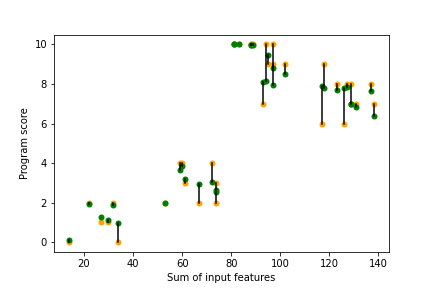
\includegraphics[scale=1.0]{./figures/ss_rf.png}
\caption{Actual score vs score predicted by Random Forest Regressor}
\label{fig_rf}
\end{figure}

\begin{figure}[H]
\centering
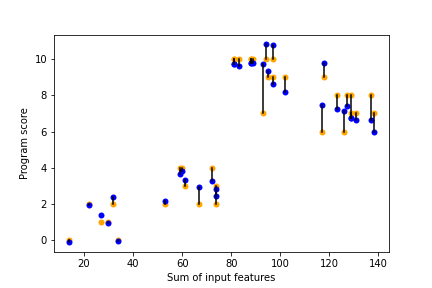
\includegraphics[scale=1.0]{./figures/ss_svr.png}
\caption{Actual score vs score predicted by Support Vector Regressor}
\label{fig_rf}
\end{figure}

\begin{figure}[H]
\centering
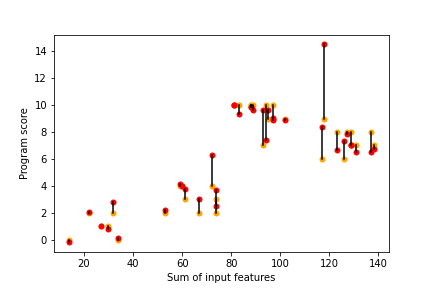
\includegraphics[scale=1.0]{./figures/ss_mlp.png}
\caption{Actual score vs score predicted by Multi Layer Perceptron Regressor}
\label{fig_rf}
\end{figure}

While multi-layer perceptron regressor and linear support vector
regressor can output a score greater than 10 or lesser than 0, random
forest regressor always outputs a score in the range of 0 to 10. This
characteristic of random forest regressor is accounted by the decision
trees which form the regressor. Since MLP regressor trains through
backpropagation and support vector regressor tries to find the best
hyperplane which contains maximum number of points, these models may
output a score greater than 10. But in the case of random forest
regressor, the model outputs a score based on the ensembling of
various decision trees. The maximum score that can be awarded will be
set as 10 and when a particular code submission passes all conditions
(conditions are based on different feature values), that program will
be graded with a score of 10.

This can be observed in Figures 7.1 to 7.3. In case of random forest
regressor, as shown in Figure~7.1, the scores always lie between 0 and
10. Also, the difference between actual and predicted values is lesser
in general. In case of Support Vector Regressor, as shown in Figure
7.2, a couple of samples were given a score of over 10. In case of
multi layer perceptron, one code sample was given a score over 14.
So, it can be inferred that Random Forest regressor is the most suited
regression model for automatic grading of student programs.




\chapter{FEEDBACK GENERATION}

After prioritizing the best regression models for each problem, we
move on to using the selected model for generating feedback. The
feedback generation process follows a cyclic information flow where
the model is verified each time for a change depending on the input
change and the corresponding change is reflected as feedback. The
following subsections explain the process of how constructive feedback
is generated.

\section{GOLDEN FEATURE VECTOR}

The golden feature vector $F$ is the best feature vector that is
calculated for each problem. In retrospect, the golden feature vector
is the average of feature vectors of all code solutions submitted for
the program that have score greater than or equal to an empirically
decided threshold.

At any instance, the golden feature vector represents the correct and
accurate code solutions for a particular problem. The goal of this
vector is to act as a comparison tool for feature vectors that require
feedback/improvement.

\section{ALGORITHM}

Now, to generate feedback for a particular target program $x$ with
$x_{i}$ features where 'i' ranges between 0 to 17, we perform an iterative process of replacing one of the
features $x_{i}$ with the corresponding feature value $X_{i}$ from the
program's golden feature vector $F$. Now, the new modified feature
vector is passed as input into the regression model.

\begin{itemize}
\item If the output score improves after replacement, now we compare
  $x_{i}$ and $X_{i}$.
  \begin{itemize}
  \item If $x_{i} > X_{i}$, it is advised to decrease that feature in the program.
  \item If $x_{i}<X_{i}$, it is advised to decrease that feature in the program.
  \end{itemize}
\item If the output score decreases after replacement, we consider the
  next feature in $x_{i}$
\item The above process is iterated until all the n features have been
  considered.
\end{itemize}

In each iteration, the goal of the algorithm is to make the target
feature vector closer to the golden feature vector. Thus, the changes
that are suggested as feedback are inferred to be improvements
for the target vector and constructive feedback is provided.


\chapter{DEPLOYMENT}

After the regressor model for automatic grading and feedback generation was finalised as Random Forest Regressor (which in general outperformed the other two models), the next step was to deploy the model with a user interface where students can login and attempt the tasks. Once the students submit their solution, the score for their submission and feedbacks if any had to be displayed.

Streamlit framework was used to deploy the random forest regressor model which would grade students' code solution submissions out of 10 and to generate appropriate feedbacks. Streamlit framework was chosen since it provides a variety of advantages. Firstly, it is simple to create web applications with few lines of python code using Streamlit. It supports a lot of python frameworks and libraries like pandas, numpy, scikit-learn, Pytorch, Tensorflow etc.

Another big advantage of Streamlit is that it provides a mechanism for caching - so that even when a expensive computation is done or a large dataset is manipulated, the app's performance will not be compromised.
This is achieved with the use of the st.cache decorator.

Sqlite3 database was integrated with the web application so that new students can register and existing students can login to the student code submission portal. 



\newpage
\begin{figure}[h]
\centering
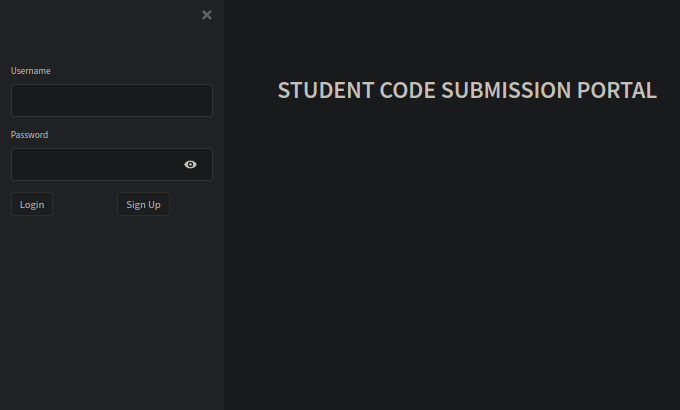
\includegraphics[scale=0.6]{./figures/dep1.png}
\caption{Snippet of Student Code Submission portal before login}
\label{fig1}
\end{figure}

\begin{figure}[h!]
\centering
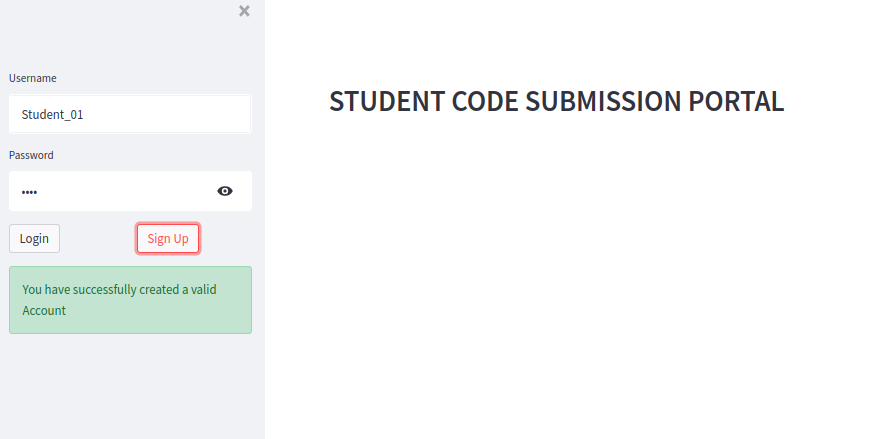
\includegraphics[scale=0.5]{./figures/dep2.png}
\caption{Snippet of Student Code Submission portal after login}
\label{fig2}
\end{figure}

\newpage
\newpage
Figure 9.1 is the snippet of the student code submission portal before login. Since the student has not logged in yet, the tasks to be attempted are not visible.

Figure 9.2 is the snippet of the student code submission portal after login. Once the student enters his username and password, the password is hashed using Secure Hash Algorithm (SHA 256) and the system checks if the user has registered already. Post successful login, the select-box and code area become visible to the student.  



\begin{figure}[h!]
\centering
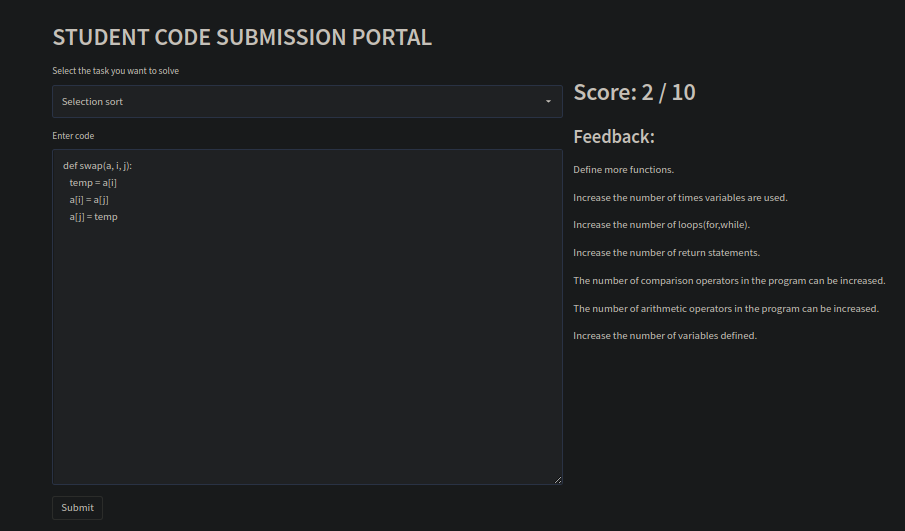
\includegraphics[scale=0.5]{./figures/dep3.png}
\caption{Automatic Grading and Feedback Generation - Example 1}
\label{fig3}
\end{figure}

Figure 9.3 shows a example student submission for the selection sort task. Since the code is incomplete and only swap function is defined, the code submission is given a score of 2 out of 10. The code review feedbacks which are generated are appropriate which include suggestions like to define more functions, add more looping statements etc.

\newpage

\begin{figure}[h!]
\centering
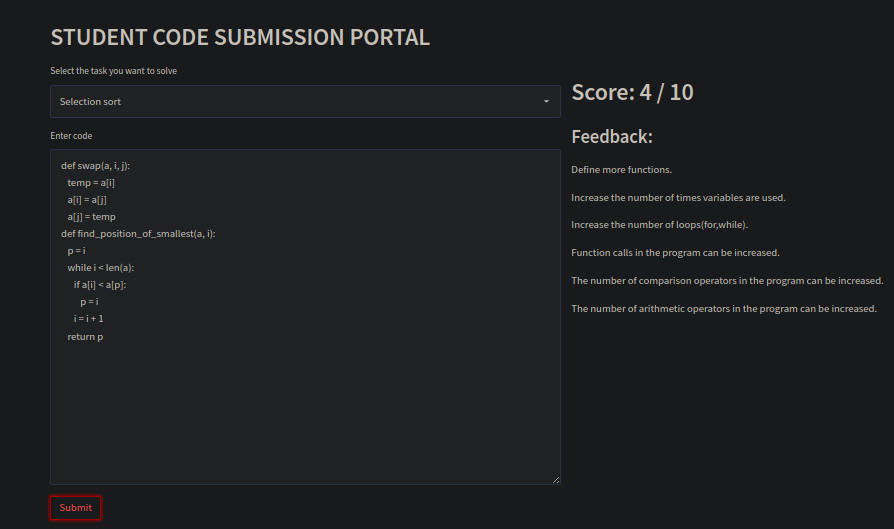
\includegraphics[scale=0.5]{./figures/dep4.png}
\caption{Automatic Grading and Feedback Generation - Example 2}
\label{fig4}
\end{figure}

Figure 9.4 shows another example student submission for the election sort task. In this case, the program is incomplete again - with only two functions defined for swapping and finding the position of the smallest element in the list from a given index. Since the main sort function is missing which would have had function calls to the two defined functions and a looping statement, the code submission gets a grade of 4 out of 10 and the necessary code review feedbacks.

Figure 9.5 is another example student submission for selection sort task. In this case, the model grades the program a perfect 10/10 with no code review feedbacks. The code submission is perfect with three functions defined to perform swapping, finding the position of the smallest element from a given index and finally the sort function. The sort function includes two function calls to the previously defined functions. Thus, the model considers the particular code submission as a perfect code sample. 

\newpage

\begin{figure}[h!]
\centering
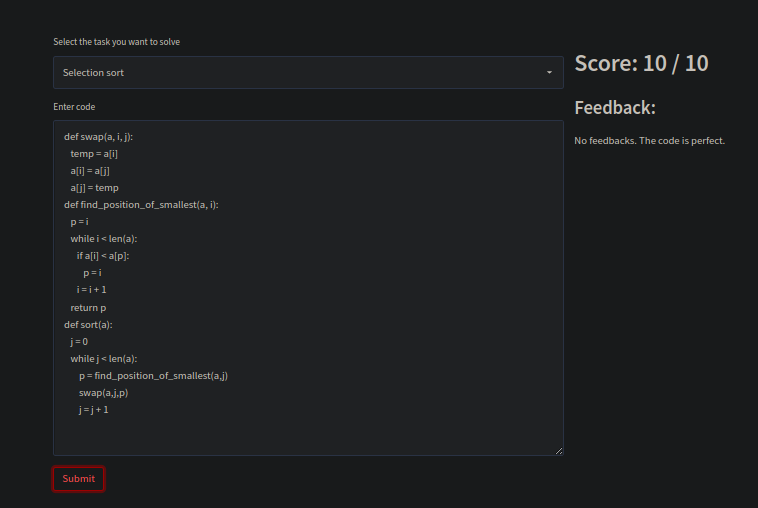
\includegraphics[scale=0.6]{./figures/dep5.png}
\caption{Automatic Grading and Feedback Generation - Example 3}
\label{fig5}
\end{figure}



\chapter{CONCLUSION}

We proposed a pipeline for grading a student code submission out of 10
which will also provide appropriate feedback to improve the code. The
features were retrieved from both the source code and the AST
representation of the source code. The feature set for each coding
assignment was optimised via feature selection. The initial dataset
created by us was used to train three regressor models such as Support
Vector regressor, Multi Layer Perceptron regressor and Random Forest
Regressor. The Random Forest regressor was shown to be the most
effective for this issue statement. The Random Forest Regressor model
has a MAE of 1.7 and RMSE of 2.3.

Furthermore, depending on the difference between a program's feature
values and the average feature values of ``excellent'' programs, our
model provides personalised feedback.  Whenever a student submits a
code, he will be given feedback instantly to help him improve his
code.  Students can also view the best code submission after the
assignment deadline. The Streamlit framework was used to deploy this
pipeline as a web app.

\end{spacing}
\newpage
\appendix
%\addtotoc{REFERENCES}
%\input{References} 
%\bibliographystyle{plain}
%\bibliography{ref}
\begin{thebibliography}{99}
  \bibliographystyle{apa}
  
\bibitem[1]{G} ``2to3 -- Automated Python 2to3 code translation'', https://docs.python.org/3/library/2to3.html 

\bibitem[2]{F} ``AST module Python 3.10.4'', https://docs.python.org/3/library/ast.html
  
\bibitem[3]{A} Azcona D, Arora P, Hsiao I H, Smeaton
  A. (2019) ``user2code2vec: Embeddings for profiling students
  based on distributional representations of source code'' ,
  In Proceedings of the 9th International Conference on
  Learning Analytics \& Knowledge, pp. 86-95.

\bibitem[4]{O} Benjamin Paaben, Barbara Hammer, Thomas
  William Price, Tiffany Barnes, Sebastian Gross, and Niels
  Pinkwart. (2017) ``The Continuous Hint Factory-Providing
  Hints in Vast and Sparsely Populated Edit Distance Spaces'',
  arXiv preprint arXiv:1708.06564

\bibitem[5]{B} Breiman L. (2001). ``Random forests --- Machine
  Learning'' 45, 5-32.

\bibitem[6]{N} Chris Piech, Jonathan Huang, Andy Nguyen, Mike
  Phulsuksombati, Mehran Sahami, Leonidas Guibas. (2015)
  ``Learning program embeddings to propagate feedback on
  student code'' , In Proceedings of the 32nd International
  Conference on International Conference on Machine
  Learning-Volume 37. JMLR. org, 1093–1102.

\bibitem[7]{D} Drucker, Harris, et al. (1996) ``Support
  vector regression machines'', Advances in neural
  information processing systems, 9.

\bibitem[8]{H} Jović, Alan, Karla Brkic, Nikola
  Bogunovic. (2015) ``A review of feature selection methods
  with applications'' , 38th international convention on
  information and communication technology, electronics and
  microelectronics (MIPRO). Ieee, 2015.

\bibitem[9]{Q} Lili Mou, Ge Li, Lu Zhang, Tao Wang, Zhi
  Jin. (2016) ``Convolutional Neural Networks over Tree
  Structures for Programming Language Processing'', In AAAI,
  Vol. 2. 4

\bibitem[10]{M} Lili Mou, Ge Li, Yuxuan Liu, Hao Peng, Zhi
  Jin, Yan Xu, Lu Zhang. (2014) ``Building program vector
  representations for deep learning'', arXiv preprint
  arXiv:1409.3358.

\bibitem[11]{J} Maxim Rabinovich, Mitchell Stern, Dan
  Klein. (2017) ``Abstract syntax networks for code
  generation and semantic parsing'', arXiv preprint
  arXiv:1704.07535.

\bibitem[12]{L} Miltiadis Allamanis, Hao Peng, Charles
  Sutton. (2016) ``A convolutional attention network for
  extreme summarization of source code'', In International
  Conference on Machine Learning. 2091–2100.

\bibitem[13]{C} Murtagh, Fionn. (1991) ``Multilayer
  perceptrons for classification and regression''
  ,Neurocomputing 2.5-6 : 183-197.

\bibitem[14]{T}Orr, J Walker, Nathaniel Russell. (2021)
  ``Automatic Assessment of the Design Quality of Python
  Programs with Personalized Feedback'', arXiv preprint
  arXiv:2106.01399 .

\bibitem[15]{E} Pedregosa et al., (2011) ``Scikit-learn:
  Machine Learning in Python'', JMLR 12, pp. 2825-2830.

\bibitem[16]{S} Pylint.org. ``Pylint - code analysis for
  python''. https://pylint.org.

\bibitem[17]{P} Sebastian Gross, Bassam Mokbel, Benjamin
  Paaben, Barbara Hammer, Niels Pinkwart. (2014)
  ``Example-based feedback provision using structured
  solution spaces'', International Journal of Learning
  Technology 10 9, 3 , 248–280.

\bibitem[18]{R} Sebastian Proksch, Sven Amann, Sarah Nadi,
  Mira Mezini. (2016) ``A dataset of simplified syntax trees
  for C'', In Proceedings of the 13th International
  Conference on Mining Software Repositories. ACM, 476–479.

\bibitem[19]{I} Uri Alon, Meital Zilberstein, Omer Levy, Eran
  Yahav. (2018) ``A general path-based representation for
  predicting program properties'', arXiv preprint
  arXiv:1803.09544.

\bibitem[20]{K} Veselin Raychev, Martin Vechev, Eran
  Yahav. (2014). ``Code completion with statistical language
  models'',In Acm Sigplan Notices, Vol. 49. ACM, 419–428.

\end{thebibliography}


\end{document}
`
